\setchapterpreamble[u]{\margintoc}
\chapter{Neutrinos in IceCube} 
\labch{nu_icecube}



The theoretical discussions from the previous chapters showed how neutrinos are essential for comprehending the origin of cosmic rays, as they serve as clear evidence of particle acceleration and hadronic interactions. However, detecting astrophysical neutrinos is highly challenging due to their small interaction cross-sections and the low fluxes expected from astrophysical objects at Earth. In short, a large detection volume is necessary. In this chapter, the entire process of neutrino detection will be described from the secondary particles produced in neutrino interactions to the propagation of their Cherenkov light in ice to the recording of this light with IceCube’s optical sensors.


\section{IceCube Neutrino Observatory}
\label{sec:IC_detector}
As described in \ref{sec:nu_interactions},the detection of high-energy neutrinos requires a large detector due to their small interaction cross-section. When these neutrinos interact, the secondaries produce Cherenkov photons (see \ref{sec:cherenkov}), therefore, the detector must be transparent to these photons. Such a large detector volume can be acquired by using natural resources such as large bodies of water or ice; by deploying photosensors underneath to create a sufficiently sized detector.\par
This concept was first introduced in 1960 \sidecite{Markov:1960vja}. The groundwork for implementing such a detector began with water-based experiments like DUMAND \sidecite{PhysRevD.42.3613}, which was planned to be deployed in the sea near the main island of Hawaii and another detector with a similar design Lake Baikal \sidecite{BELOLAPTIKOV1997263}. First ever large-scale neutrino telescope built was predecessor of IceCube experiment called AMANDA \sidecite{ANDRES20001} at the geographic South Pole. A few hundred optical modules were dropped under the ice sheet of this dry continent between the depth of 1.5 to 2 km. Needless to say, the IceCube detector, the largest neutrino telescope in the world today, benefitted greatly in terms of design and performance from all the research and development work that was done with AMANDA. 
There also exists a large volume water-based neutrino telescope in the Northern Hemisphere called ANTARES\sidecite{AGERON201111}, and its successor KM3NeT\sidecite{MARGIOTTA201483}, located in the Mediterranean Sea.\par
The following subsections will discuss various detector and hardware components of the IceCube detector. Additionally, the last section will cover the optical properties of the South Pole ice, as these properties strongly affect the analysis observable and therefore influence the flavor measurements presented in this thesis.\par


\subsection{Detector}
\label{sec:IC_coordinate}
\begin{figure}
	\centering 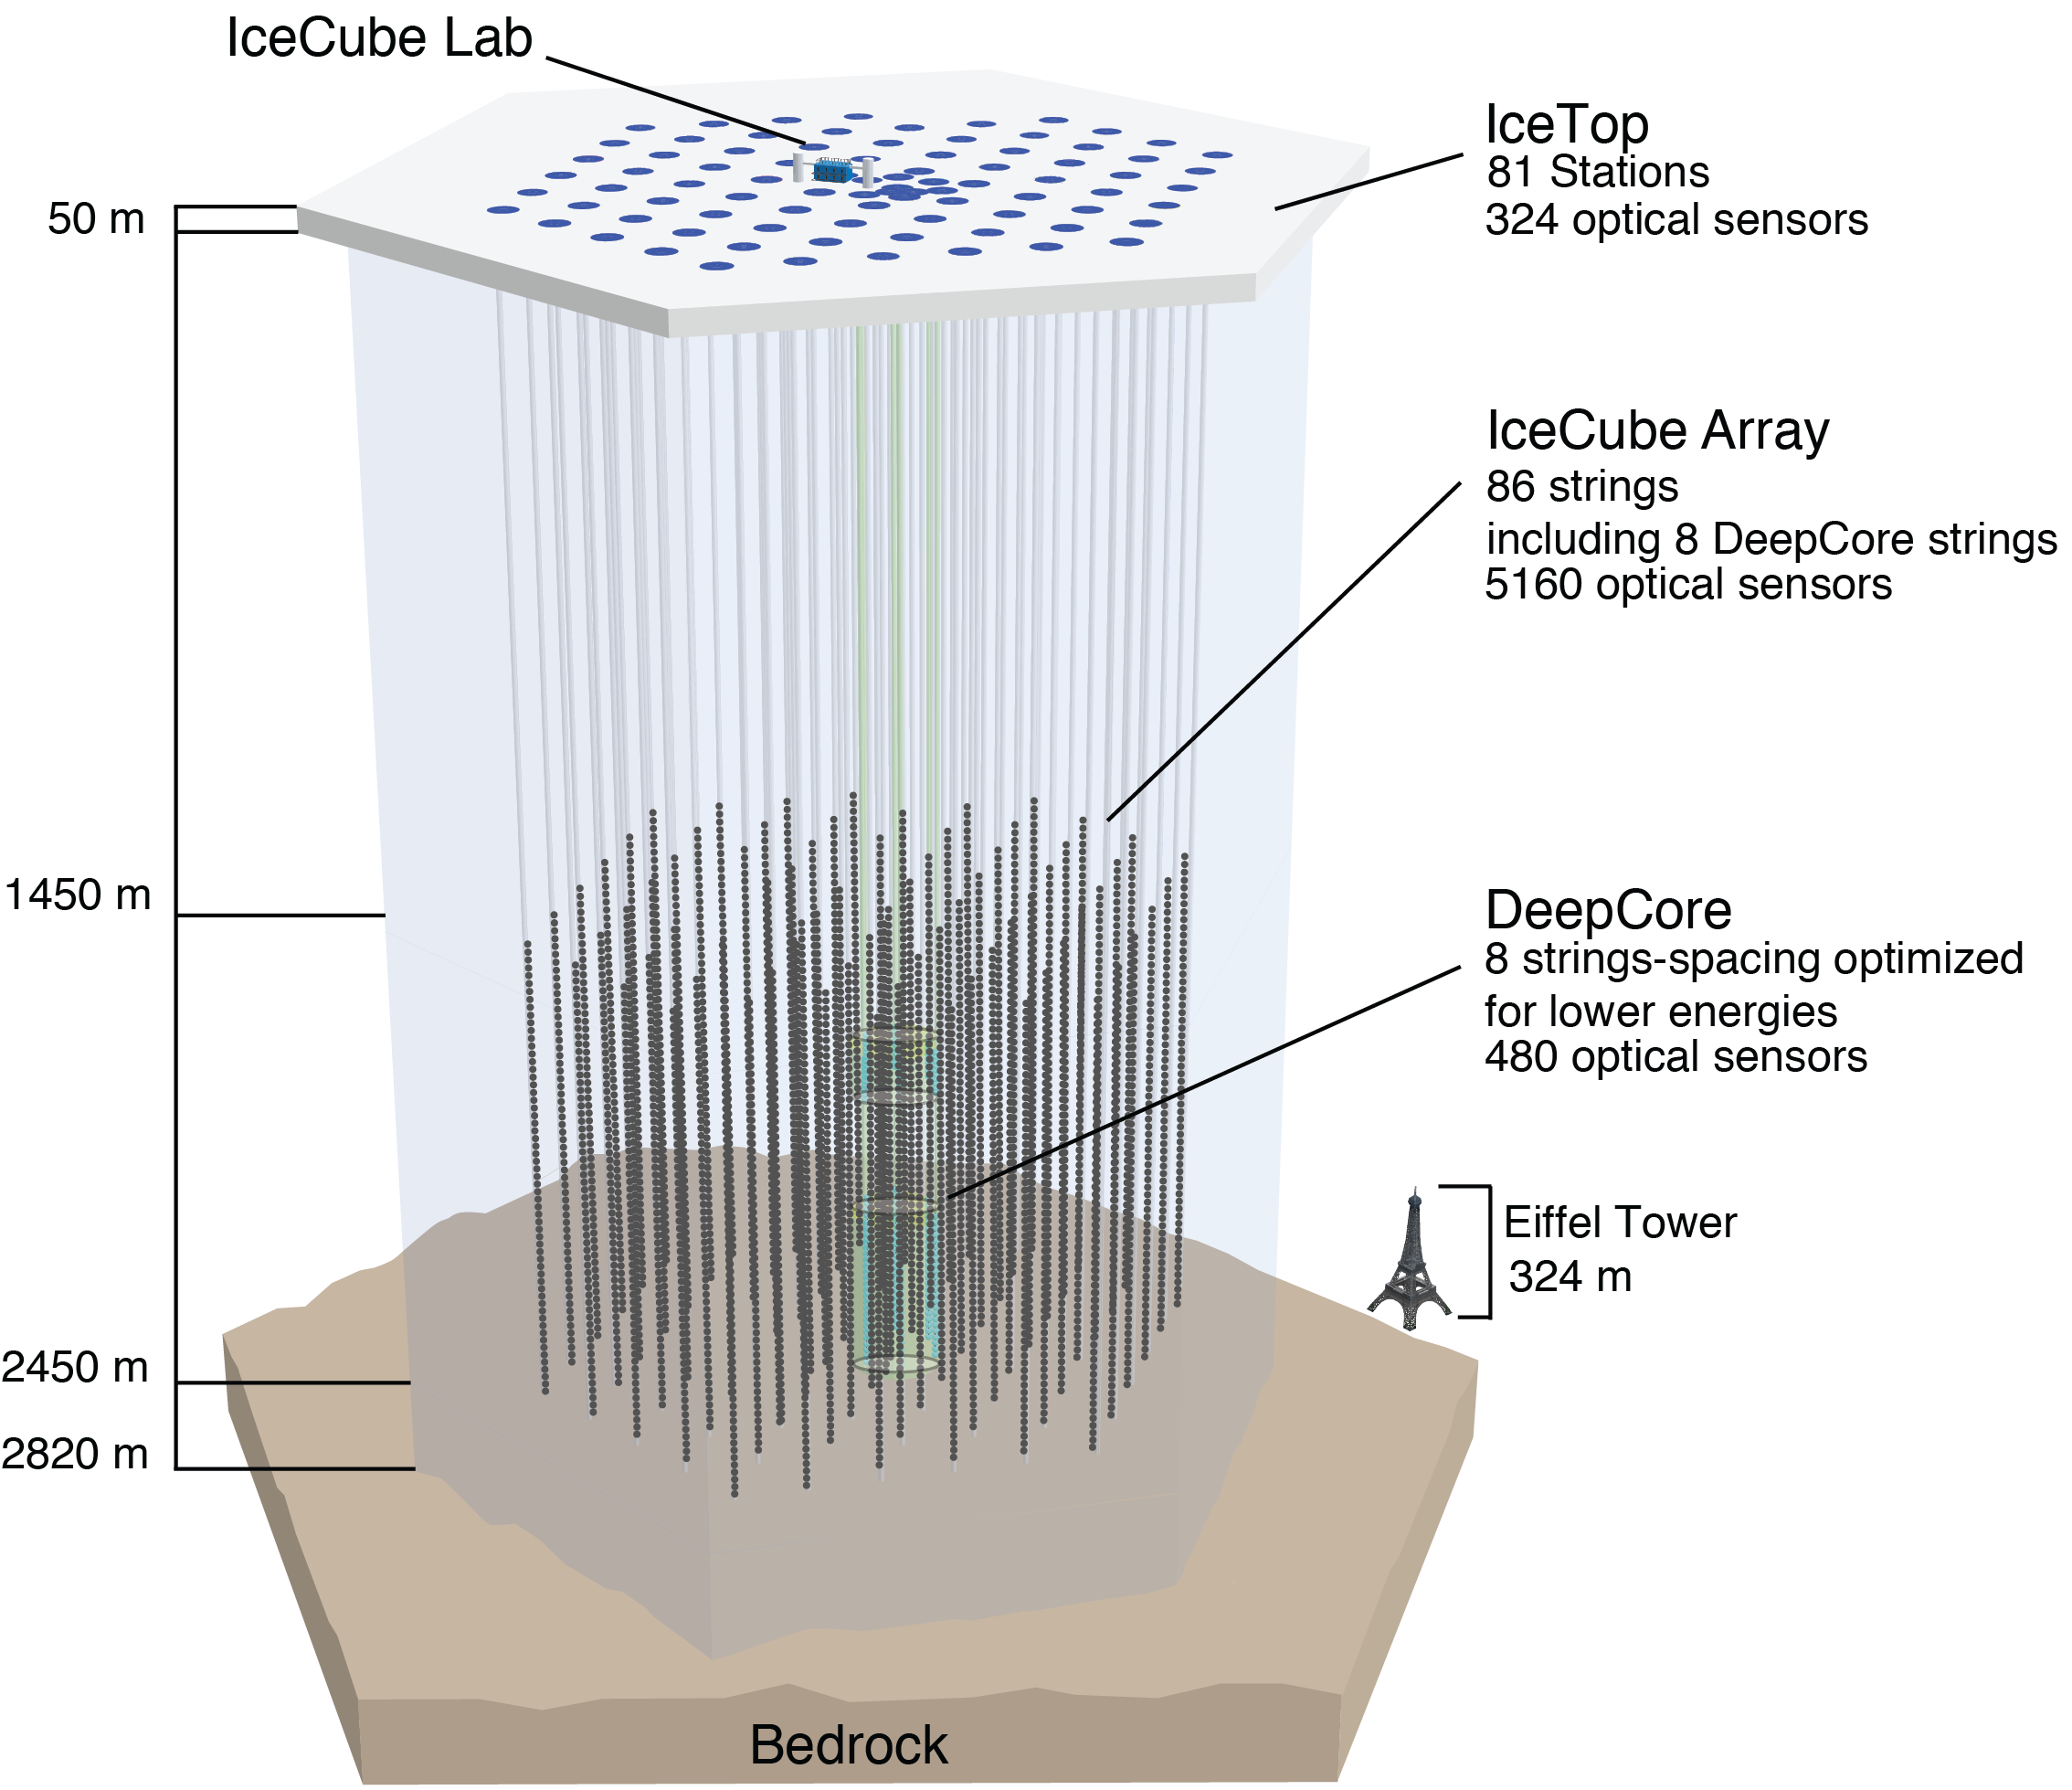
\includegraphics{./figures/nu_in_icecube/IceCubeArray_slim.png}
	\caption{A schematic overview of the IceCube detector and its components \cite{Aartsen_2017}}
    \labfig{ic_detector}
\end{figure}
    
\begin{marginfigure}
	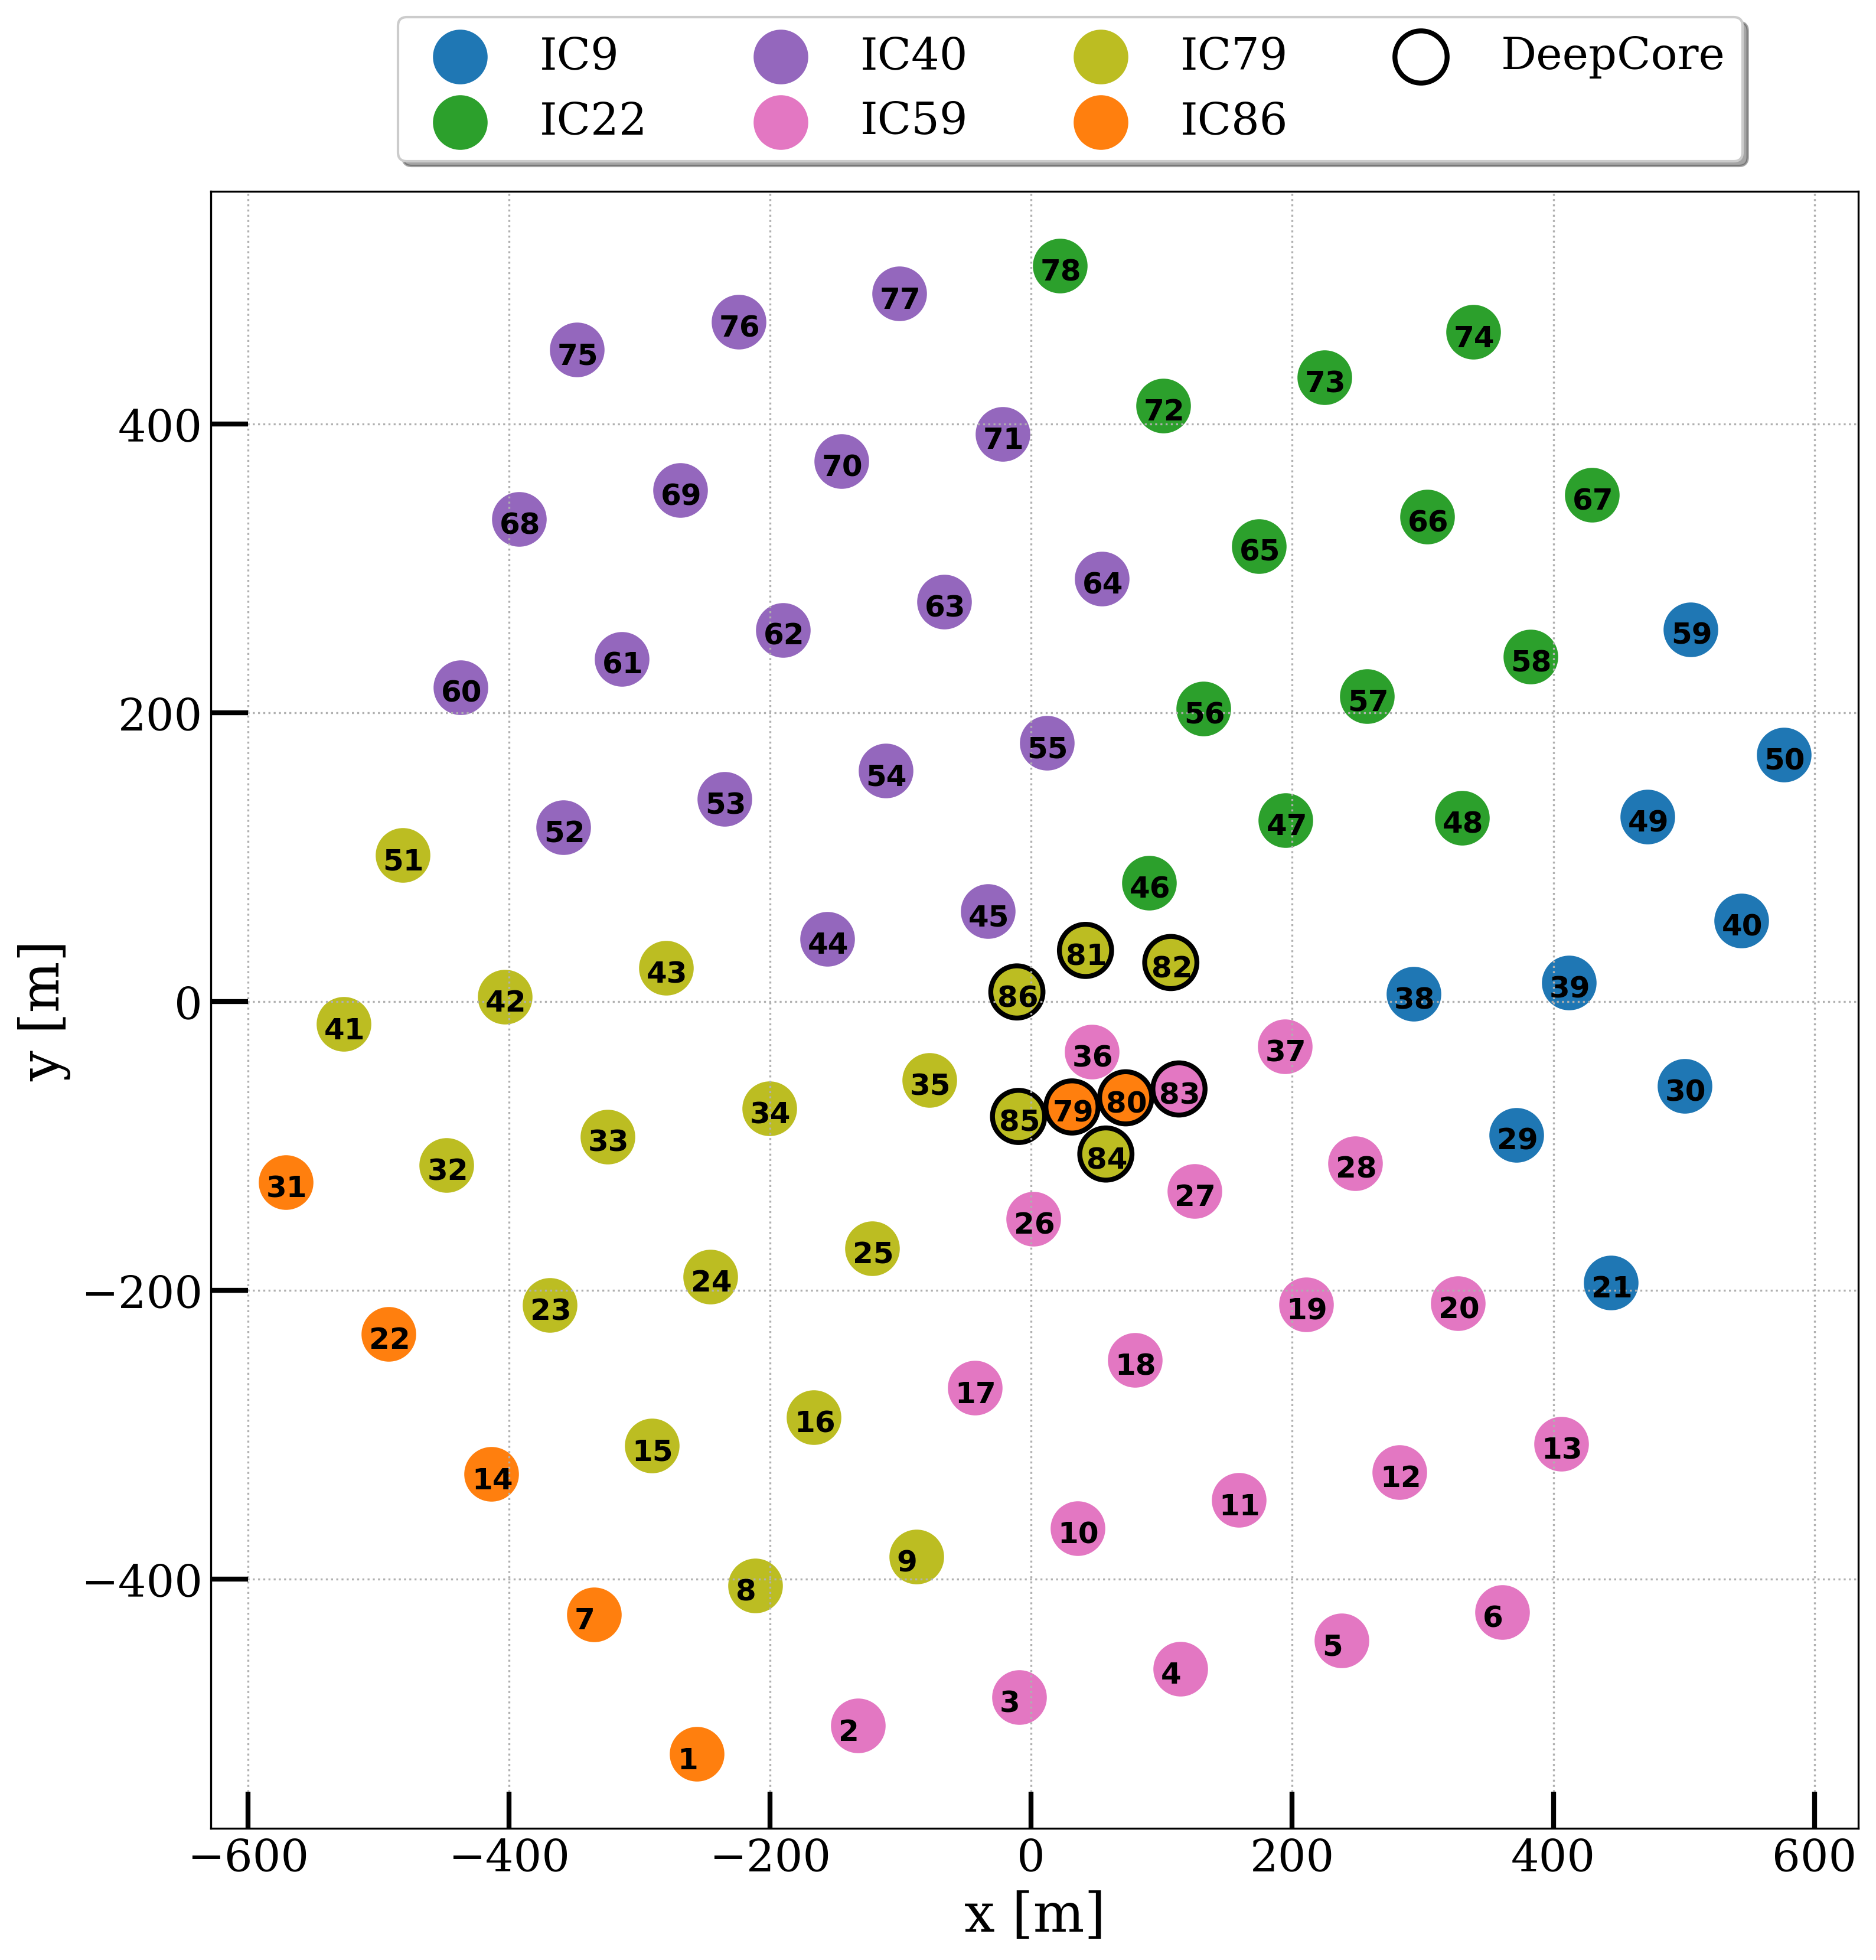
\includegraphics{./figures/nu_in_icecube/IC_Phase_Array.png}
	\caption{Top view of the location of each \emph{in-ice} strings of IceCube. Colour represents set of strings deployed in each seasons as described in \reftab{deployment_phases}. Note: IceTop Stations are not shown here.}
	\labfig{ic_phase_array}
\end{marginfigure}

\textbf{The IceCube Neutrino Observatory} is located at Amundsen-Scott South Pole Station at the geographic South Pole. It comprises a cubic kilometer of instrumented ice, equipped with 5,160 digital optical modules reffered as \emph{DOMs} from here-on (see \ref{sec:dom}), buried deep in the ice and 81 IceTop Stations on the surface of the ice, making itself the largest Neutrino Observatory in the world \sidecite{Aartsen_2017}. A schematic of the detector layout is shown in \reffig{ic_detector}. Four main components of the detector are \emph{in-ice array,DeepCore (inner extension of in-ice array),IceTop and IceCube Lab}. \par

\begin{description}
	\item[The Main \emph{in-ice} array] consists of 78 strings,\marginnote
    {\begin{kaobox}[title=\textbf{\emph{string} in IceCube}]
        An arrangement of DOMs attached on a twisted copper wire cable makes the so-called \emph{string} in IceCube.
    \end{kaobox}}
    each consisting of 60 DOMs, spaced vertically at a distance of 17 m between the depth of 1450 m to 2450 m under the ice sheet of Antarctica. Horizontal spacing between each of these strings is 125 m.  
	\item[\emph{DeepCore}] comprises inner 8 strings (see \reffig{ic_phase_array}) of the main\emph{in-ice} array, placed more closely together with horizontal string distance of 70 m and vertical DOM distance of 7 m \sidecite{deepcoredesign} between 1750 m to 2450 m depth. There's a region between depth of 1850 m to 2100 m, with no DOMs attached to the string as this region is the so-called \emph{dust layer} (see section \ref{sec:icemodel}), where optical scattering and absorprion is quite high and thus is not efficient to make reliable physics measurements. The Photomultipliers used in DOMs attached on these 7 strings also have higher Quantum Efficiency, which reduces the energy threshold to ~10 GeV. Although, IceCube's main goal is to detect astrophysical neutrinos, current topics of research spans much broader range (e.g fundamental properties of the neutrinos, such as oscillations \sidecite{Aartsen_2019_oscillations}, Physics beyond Standard Model searches such as Dark Matter \sidecite{Abbasi_2022} etc). 
	\item[\emph{IceTop}] is the surface detector array of the IceCube detector, primarily designed to detect Cosmic-ray airshowers and to be used as a veto layer for downgoing muons produced in these airshowers \sidecite{ABBASI2013188}. It consists of 81 \emph{stations} each having 2 tanks filled with clear ice (162 tanks in total). Each of these 162 tanks have 2 DOMs, similar to the ones deployed in \emph{in-ice} array, which makes it easier for both arrays to have a similar trigger and data acquistion system.
	\item[\emph{IceCube Lab}(ICL)] serves as the central operations' hub for the experiment, providing a crucial support for data acquisition and filtering. All the string cables connected to the aforementioned detcetor components are routed up to the ICL, from where triggered data is sent back to the northern hemispher via a satellite. Various other operations such as mainting the detector operations etc are also maintained from this building. 
	\end{description}

For the work presented in this thesis, neither \emph{deepcore} nor \emph{IceTop} data is used.
\begin{table}
    \caption{IceCube detector components deployed in each season (cumulative). Each configuration is represented as \emph{ICXX} where \emph{IC} stands for IceCube and \emph{XX} stands for number of total \emph{in-ice} strings at the end of that season}
    \labtab{deployment_phases}
    \begin{tabular}{cccc}
        \hline
        \hline
        Season & Configuration & Strings & IceTop Stations\\
        \hline
        2004-05 & IC1 & 1 & 4\\ 
        2005-06 & IC9 & 9 & 16\\ 
        2006-07 & IC22 & 22 & 26\\ 
        2007-08 & IC40 & 40 & 40\\ 
        2008-09 & IC59 & 59 & 59\\ 
        2009-10 & IC79 & 79 & 73\\ 
        2010-11 & IC86 & 86 & 81\\  
        \hline
        \hline
    \end{tabular}
    \end{table}


\marginnote{
    \begin{kaobox}[title=IceCube coordinates system]
        The IceCube coordinate system's origin is at 46500'E, 52200'N, 883.9 m elevation, which is quite close to centre of the \emph{in-ice} array. The y-axis points Grid North (toward Greenwich, UK), the x-axis points Grid East (90 degrees clockwise from North), and the z-axis points "up", forming a right-handed coordinate system.
     \end{kaobox}
    } 
The construction of the detector started taking place in 2005 and lasted for 7 Antarctic summer seasons till 2011 December. In each season, parts of the current day Hexagonal detector were deployed, as shown in \reffig{ic_phase_array} and numbers detailed in \reftab{deployment_phases}. A hot water drill was used to unfreeze the ice upto 2.5 km depth and 60 cm diameter into which these strings were then deployed (see \reffig{DOM_assembly}). The geometry of the detcetor, i.e The \emph{xy}-coordinates of the string were calculated from the drill tower position, surveyed during the deployment. Assuming the string was vertical, these coordinates were applied at all depths, with deviations of less than 1 m (later validated using the flasher data, see \ref{sec:DAQ}). Depths of the lowest DOM were determined from pressure readings, corrected for water compressibility and ambient air pressure, with vertical DOM spacings measured via laser ranger. All depths were converted to z-coordinates in the IceCube coordinate system \todo{Maybe draw a small schematic of coordinate system here next to the side note?}.\par  


\subsection{The Digital Optical Module (DOM)}
\label{sec:dom}
\textbf{The Digital Optical Module} (DOM) is a crucial component of the IceCube Neutrino Observatory, functioning as the heart of the detector. Each DOM is responsible for collecting the faint light signals produced by neutrino interactions in the Antarctic ice, amplifying these signals, and transmitting the data to the IceCube Lab \cite{Aartsen_2017}. From there, the data is relayed to the Northern Hemisphere via a satellite for further analysis. 

Inside each DOM, a 10-inch Photo Multiplier Tube (PMT) is positioned at the bottom, accompanied by essential circuitry for power conversion, data acquisition, calibration, control, and data transfer. Individual components of a DOM are as shown in \reffig{DOM_schematic}, functions of each of which is explained briefly below.

\begin{description}

    \item[Glass Vessel Properties :] The glass vessel of the DOM is engineered to withstand the extreme pressures found in the deep Antarctic ice. This includes the constant long-term pressure of about 250 bar and the temporary pressure spikes of up to 690 bar experienced during the refreezing process after deployment using a hot water drill. The vessel is composed of two 0.5-inch thick hollow glass hemispheres, which are joined together with optical glue. This design not only provides a robust and hermetic seal to protect the internal electronics but also maintains the optical clarity necessary for the PMT to function effectively. The glass material is chosen for its strength, transparency, and resistance to the harsh conditions in the ice.

    \begin{marginfigure}
        % \vspace*{4.5cm}
        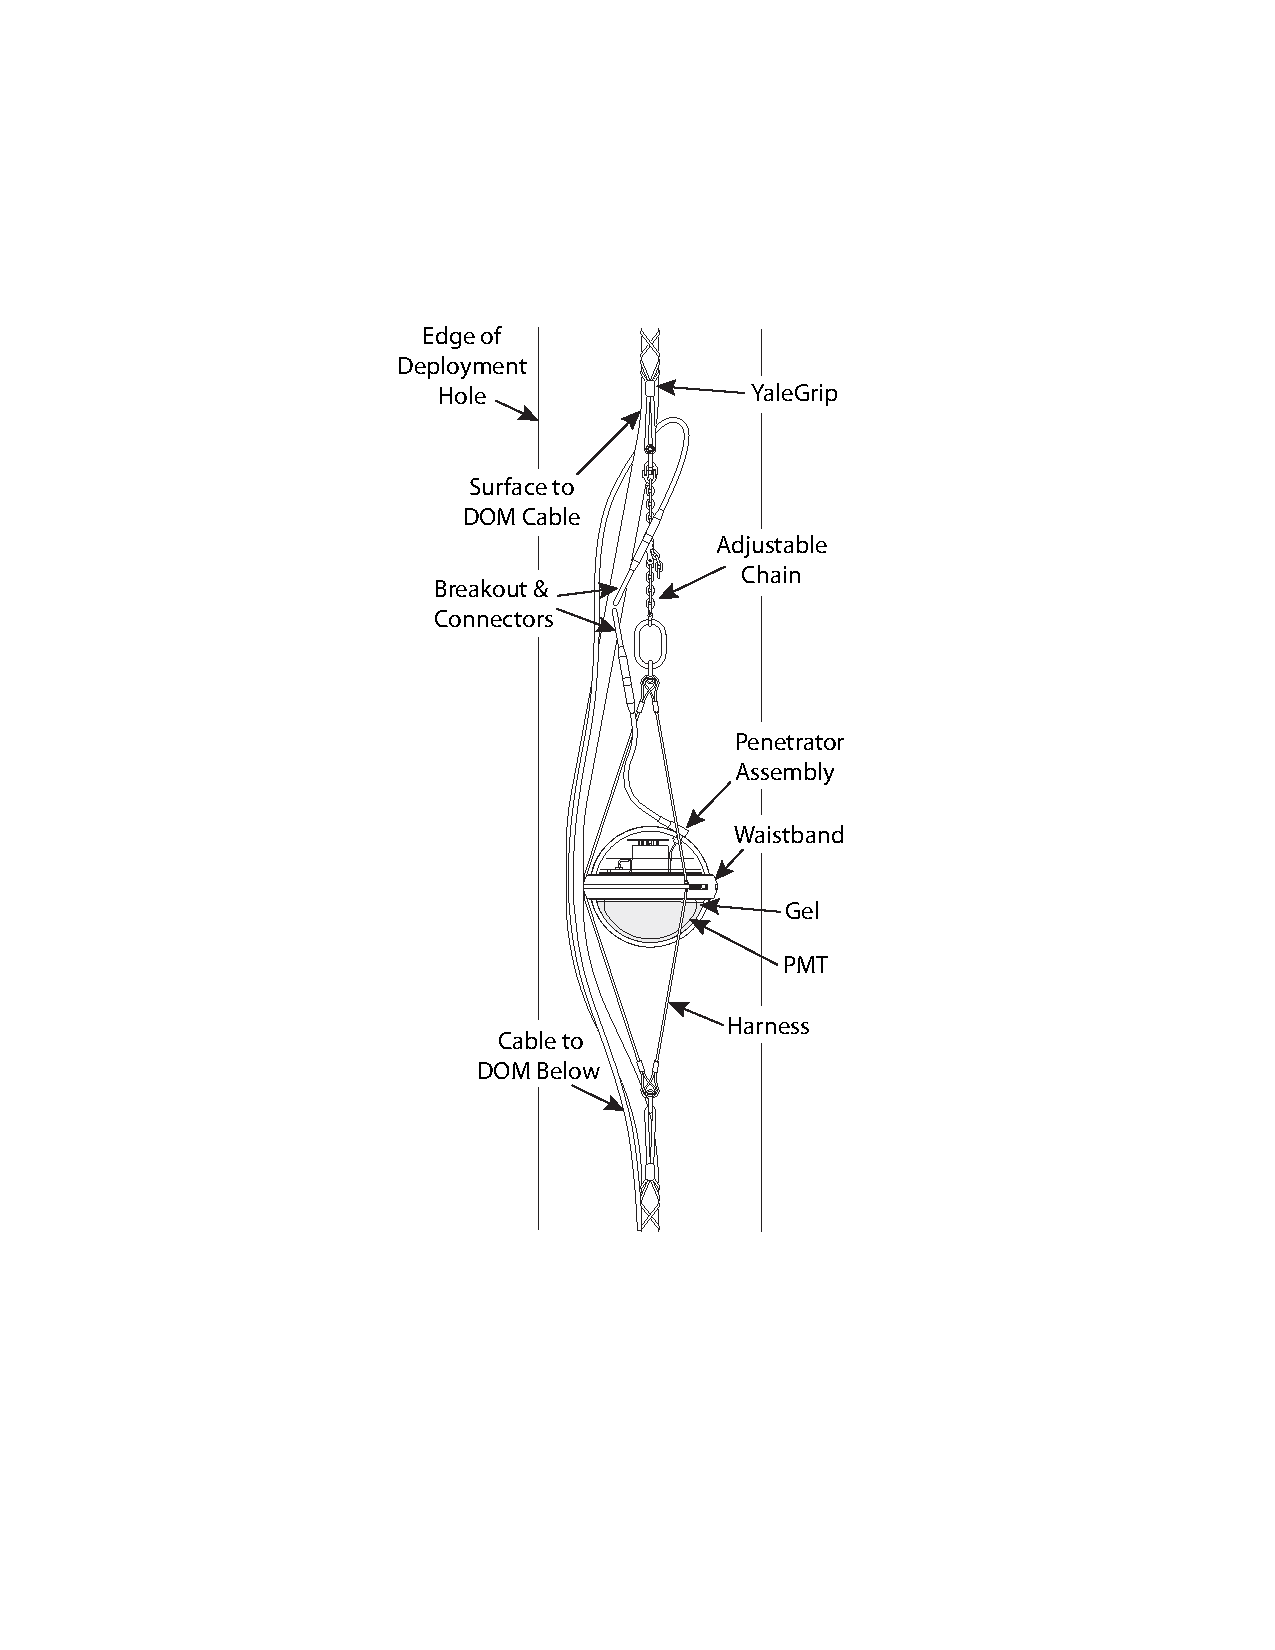
\includegraphics{./figures/nu_in_icecube/domfig2a-CableAssembly.pdf}
        \caption{A schematic of DOM CableAssembly being deployed in a water hole, created by hot water drill \cite{Aartsen_2017}.}
        \labfig{DOM_assembly}
    \end{marginfigure}
    
    \begin{marginfigure}
        % \vspace*{4.5cm}
        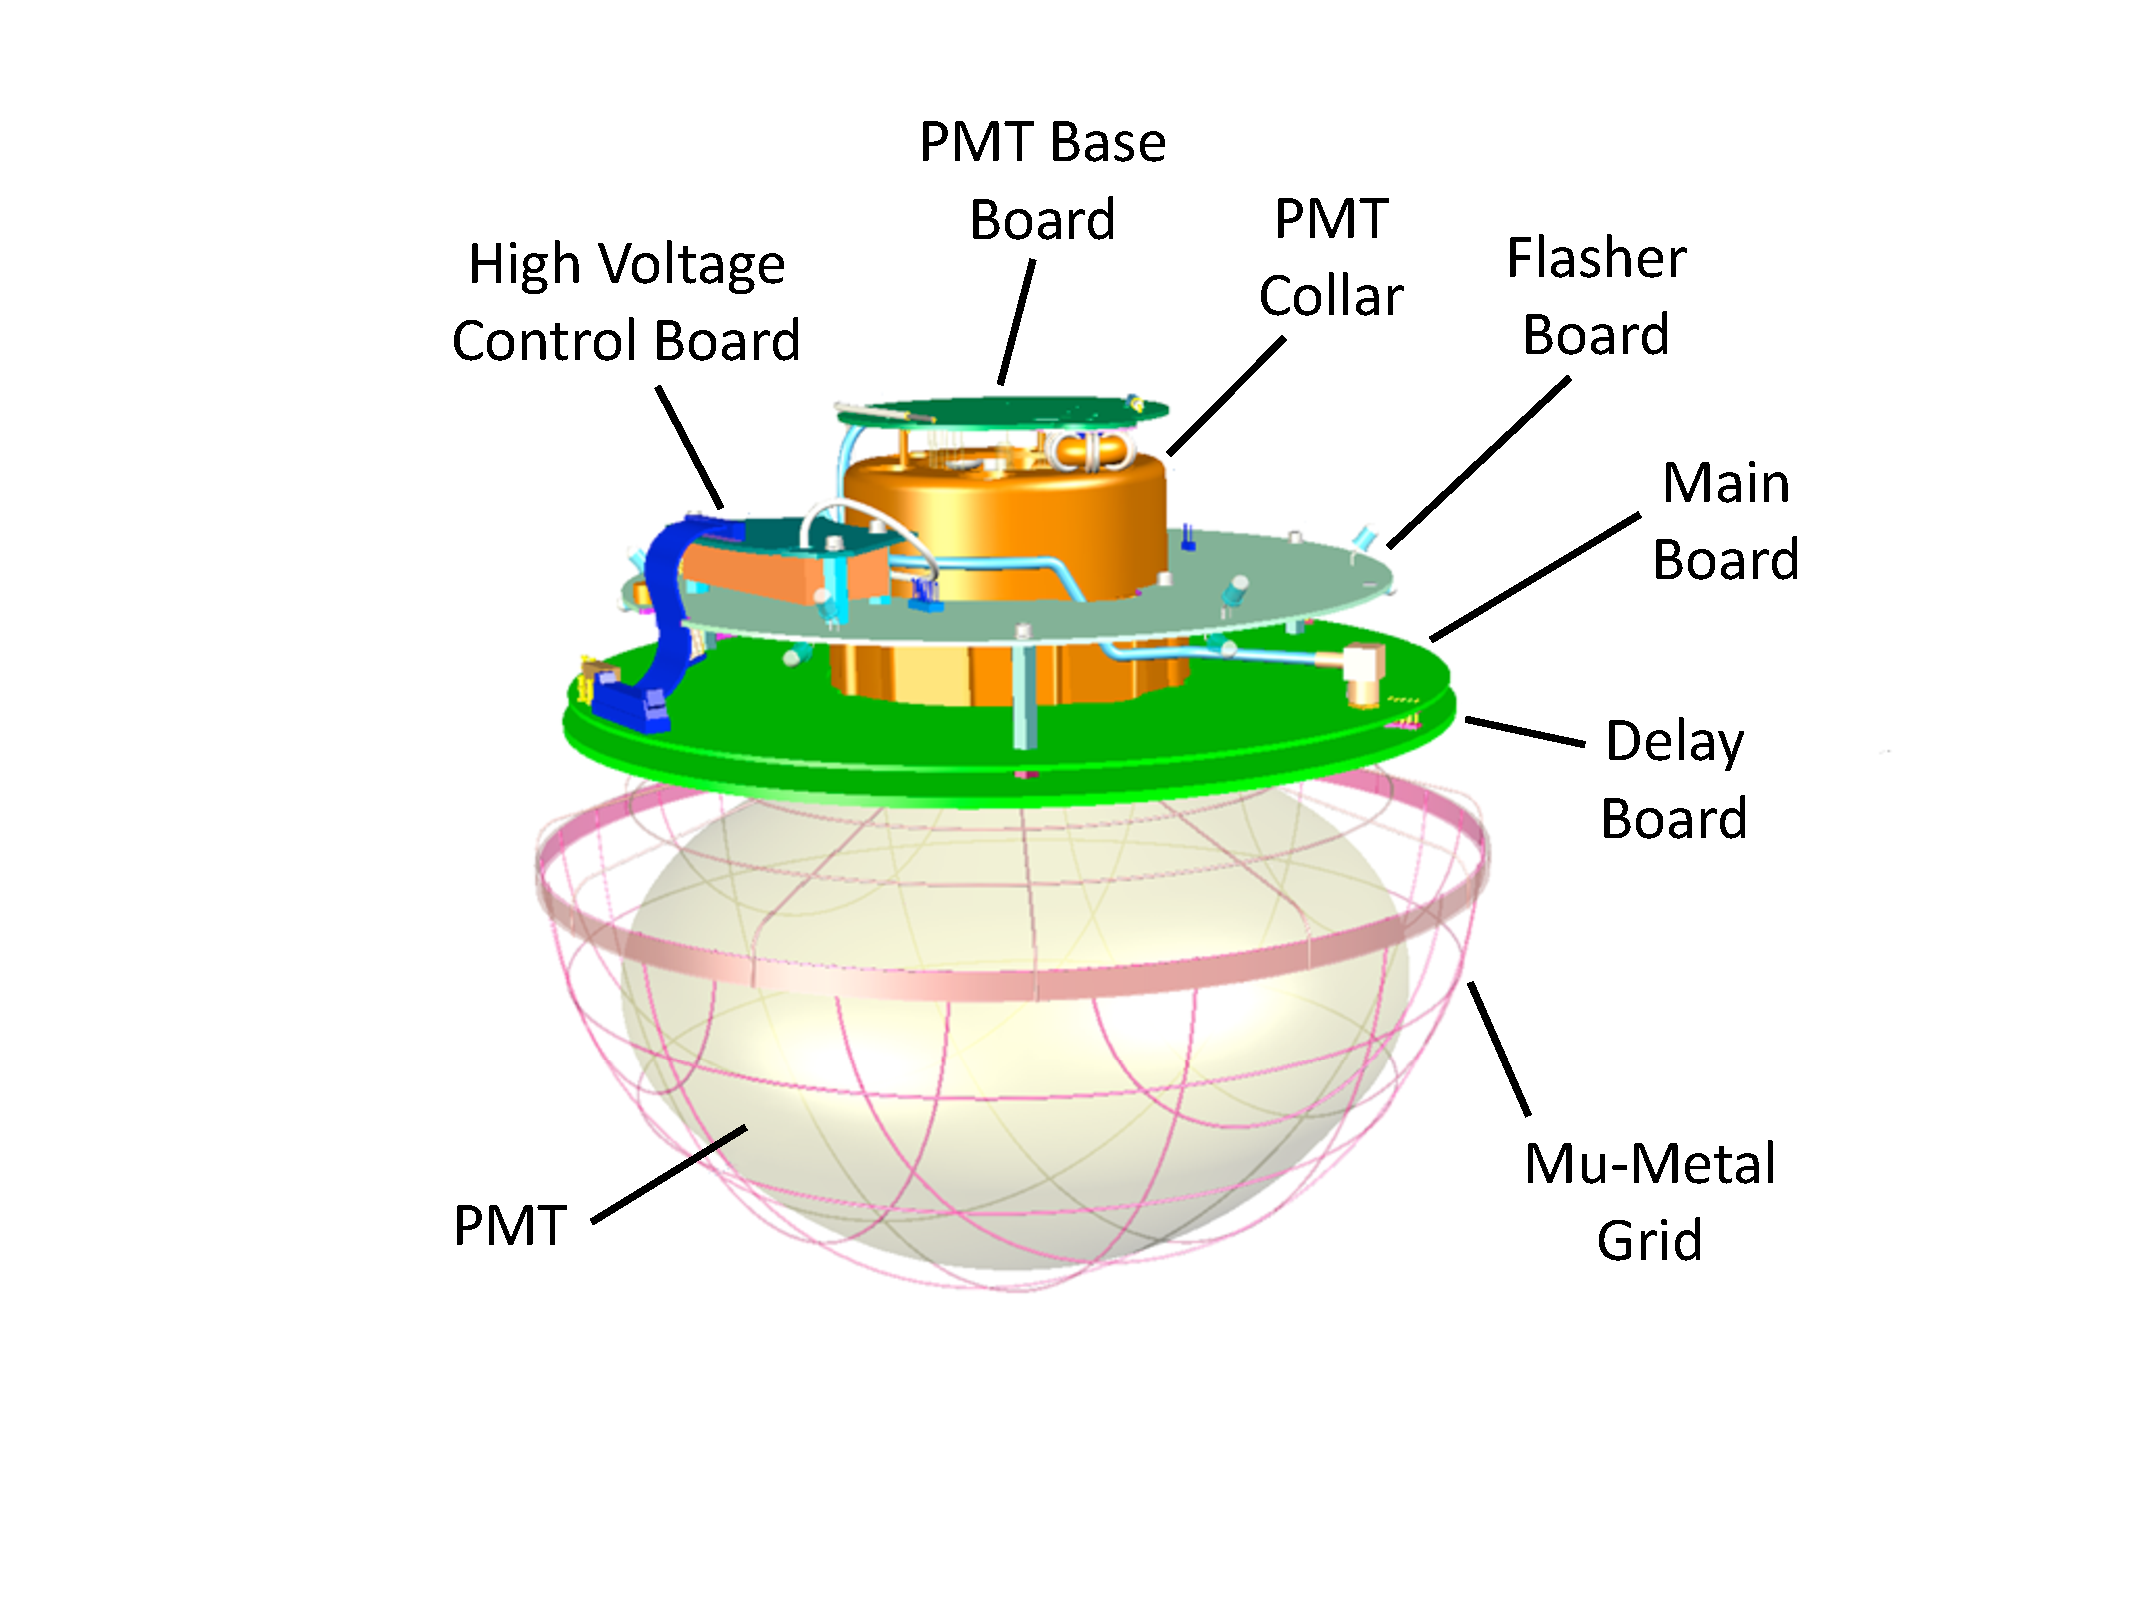
\includegraphics{./figures/nu_in_icecube/domfig1a-DOM3DModel.pdf}
        \caption{A schematic of the DOM, showing its main components \cite{Aartsen_2017}.}
        \labfig{DOM_schematic}
    \end{marginfigure}

    \item[PMT :] The PMT within the DOM is a 10-inch diameter tube that utilizes a box-and-line dynode chain with 10 stages to amplify the faint light signals detected in the ice. The PMTs used in standard in-ice DOMs have a quantum efficiency peaking at 25\% whereas, DeepCore DOMs, designed to detect lower energy neutrinos, feature PMTs with a higher peak quantum efficiency of 34\% near the 390 nm wavelength. These PMTs are operated at a gain of $10^7$.

    \item[Gel :] A high strength, silicon gel is used between the photocathode area and the glass vessel to provide optical coupling and strong mechanical support to the DOM system. This gel has a high optical clarity, with 97\% transmission at 400 nm. It shows no signs of deterioration even after a decade, ensuring reliable performance.

    \item[Magnetic Shield :] The ambient magnetic field at the South Pole, measuring around 550 milligauss (mG), angled 17 degrees from vertical, can significantly affect the performance of the PMT. This includes reducing collection efficiency by 5-10\% and causing gain variations of up to 20\%, depending on the PMT's azimuthal orientation. To mitigate these effects, a mu-metal cage is installed around the PMT bulb, extending up to its neck. This cage is constructed from a mesh of 1 mm diameter wires with a spacing of 66 mm. Although this mesh blocks about 4\% of the incident light, it substantially reduces the adverse impacts of the magnetic field, ensuring more consistent and reliable performance of the PMT.

    \item[PMT Base and High Voltage Boards :] The high voltage board includes a Digital to Analog Converter (DAC) and an Analog to Digital Converter (ADC) for precise control and monitoring of the voltages supplied to the PMT. The high voltage generator on this board provides the necessary power, which is then regulated and distributed by the voltage divider circuits on the PMT base board. These circuits are specifically designed for low power consumption, ensuring efficient and stable operation of the PMT.
    
    \item[Main Board :] The main board serves as the central processing unit (CPU) of the DOM, managing and coordinating all other electronic components. It digitizes the waveforms detected by the PMT, providing a digital representation of the light signals for further analysis. The main board also temporarily stores data, calibrates the internal clock, and exchanges local coincidence information with neighboring DOMs (see \ref{sec:DAQ}). It communicates directly with the Data Acquisition (DAQ) system, ensuring the seamless transfer of data to the IceCube Lab. Additionally, the main board hosts an adjustable low-intensity optical source, which is used to calibrate the PMT's gain and timing, ensuring consistent and accurate performance.
    
    \item[Flasher Board :] Flasher board contains 12 LEDs each having specified output wavelength of $405\pm5 \mathrm{nm}$,
    %  \marginnote{
    %     \begin{kaobox}[title="color DOMs" or CDOMs]
    %         16 of the 5160 \emph{in-ice} DOMs have multi-wavelength LEDs on their Flasher boards. 8 of these DOMs are on string 79 (quite at the centre of the detector, one of the DeepCore strings) and the other 8 on string 14 on the edge of the detector. 
    %     \end{kaobox}}
        which generates lights \emph{in situ} to make various caliberation related measurements. In addition, this board can verify timing responses (useful for many, including analysis presented in this thesis, reconstruction processes). Additionaly, to measure \emph{the optical properties} of the South Pole Ice (see section \ref{sec:icemodel}) and locations of the DOMs in ice.
    
\end{description}

\subsection{Trigger and Data Acquisition}
\label{sec:DAQ}
Ever Since the initial deployment of the first string, the detector has been consistently gathering data, maintaining an average uptime of nearly 99\% \sidecite{Abbasi_2009}. \emph{The photocathode} of the PMT of a DOM, \emph{captures} a photon which then generates \emph{photoelectrons} which are accelerated through the series of 10 dynodes to generate measurable \emph{photocurrent}. This current is integrated over a time to obtain collected charge in units of \emph{photoelectrons or PEs}, through which \emph{photovoltage} is produced at the mainboard, over time, known as \emph{waveform}. These waveforms are then digitized to acquire and relay the data to the Northern Hemisphere.

Depending on how many photons hit the PMT, these waveforms can have different amplitudes ranging from 1mV upto the linearity limit of the PMT (~2 V) in time range of 12-1500 ns. The In Order to access this rather broad dynamic range, the digitiser used, Analog Transient Waveform Digitiser (ATWD) have three channels to amplify the waveform by factor of 0.25, 2 and 16. Moreover, 2 sets of ATWD are used that can operate alternatively in order to reduce the deadtime. ATWD can digitize voltage withinn duration of 427 ns, a window sufficient to reconstruct light produced within 10s of m around a given DOM. Naturally, some photons produced in energetic interactions may travel larger distances, producing faint but detectable waveforms. To amplify and digitize these waveforms, a fast Analog to Digital Converter (fADC) is also used, together ATWD+fADC is reffered as a \emph{DOMLaunch}.

The aforementioned digitization only happens if the voltage threshold of the onboard discriminator is met, which is kept at voltage equivalent to a PE of 0.25, or in other words, a DOM is \emph{hit}. If at least two neighbouring DOMs, on the same string produces individual \emph{hits} within 1 $\mu\mathrm{s}$ called \emph{Hard Local Coincidence(HLC)}, the full \emph{DOMLaunch} is transmitted to the surface. Otherwise, only the timestamp and minimal amplitude/charge information is sent known as \emph{Soft Local Coincidence(SLC)}. The HLC condition helps reduce false triggers from PMT dark noise, which is independent across DOMs. \emph{The Data Acquisition System (DAQ)} processes further uses these HLC hits to look for temporal coincidences. Most commonly used trigger in IceCube is the so-called \emph{The Single Multiplicity Trigger (SMT-8)}, that requires eight or more HLC hits within 5 $\mu\mathrm{s}$ timewindow. If and when SMT8 trigger conditions are met, all launches (HLC and SLC) are combined into what is called an \emph{event}. 

Various algorithms are used to make an estimate of event properties such as direction, deposited energy, morphology etc. The South Pole has limited computational resources, so only simple first guess algorithms can be used there called \emph{online filters}. Processed data is transmitted to the Northern Hemisphere. After this, more sophisticated reconstruction algorithms are applied to reduce and tailor the data as per Physics analysis goal. \todo{cite simulation/reco chapter here}


\section{Optical Properties of the South Pole ice}
\label{sec:icemodel}
\begin{marginfigure}
	\centering 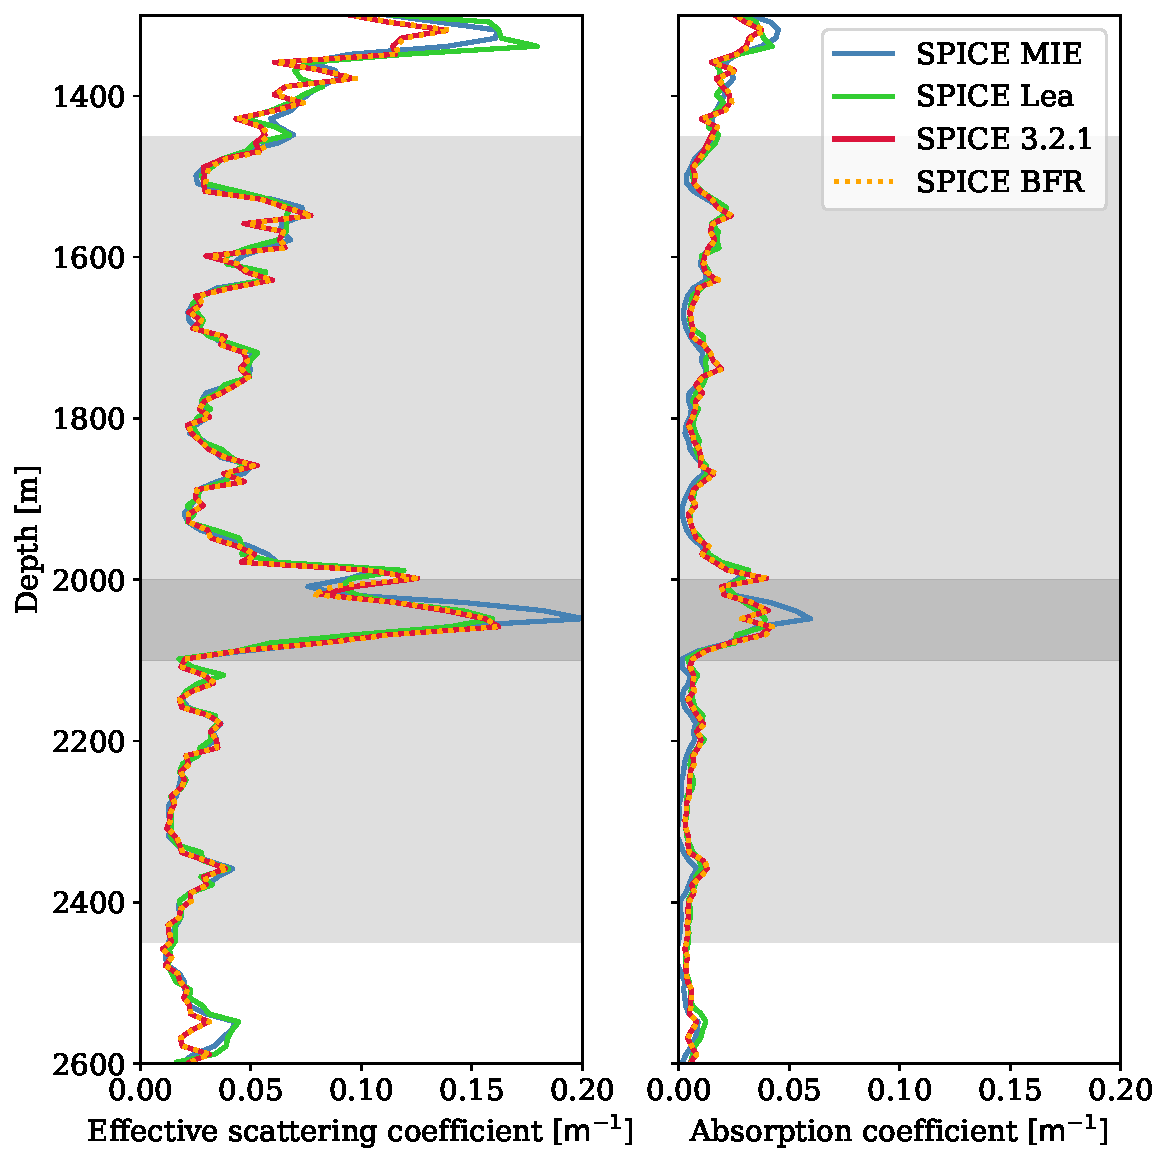
\includegraphics{./figures/nu_in_icecube/abs_scat.pdf}
	\caption{Values of effective scattering (left) and absorption (right) coefficents of 400nm photons in South Pole Ice as a function of depth, for four icemodels described in the text. Light grey area shows in-ice array and dark grey region shows the high absorption and scattering region called \emph{the dust layer}.}
    \labfig{abs_scat}
\end{marginfigure}
The ice at the South Pole is a crucial part of the IceCube detector. It acts as both the detection target and the medium through which light propagates. Unlike the DOM hardware, which has been extensively studied in the laboratory, the glacial ice can only be measured in its actual environment, making it more challenging to describe. Understanding and calibrating this medium well is essential for accurate physics measurements as photons produced from particle interactions can get absorbed or scattered from their path, making the inference of the particle interaction points challanging.

In context of Neutrino Detection, The ice at the deep South Pole was initially measured using pulsed in situ light sources (LEDs) at different wavelengths, embedded in the AMANDA array below ~1000 m depth\sidecite{optical_properties_amanda}. Later, during the construction of IceCube, direct measurements of dust concentration in the glacial ice were obtained using a dust logger deployed into some drill holes \sidecite{dust_logger}. Additionally, the LEDs on the Flasher Board of DOMs are still actively used to calibrate the detector and understand the ice properties \sidecite{spicemie}. 

\textbf{The scattering length ($\mathrm{l}_s$)} is the average distance a photon will travel before scattering off of its orignal directory. In practice, only the effective scattering length ($\mathrm{l}_\mathrm{eff}$ = $\frac{\mathrm{l}_s}{1 - \langle\cos\theta\rangle}$) can be measured, where $\langle\cos\theta\rangle$ is the average deflection angle at each scatter. \textbf{The absorption length ($\mathrm{l}_a$)} is the distance after which a photon's survival probability decreases to 1/e, indicating how far the information from an event can travel. In the case of absorption, the photon is lost, while for scattering, its direction changes, affecting both the energy and direction reconstruction of the event. Scattering and absorption parameters in \emph{ice models} are averaged over 10-meter-thick layers of ice and are calculated for a wavelength of 400 nm \cite{spicemie}. Light scattering below a depth of about $\sim$1300 m is mainly due to residual air bubbles. As depth increases, dust becomes the main source of scattering, with concentration varying due to climate and volcanic activity. At around 2000 meters, scattering and absorption significantly increase due to high dust concentration, possibly from a major volcanic eruption in the past, known in IceCube as \textbf{the dust layer} \sidecite{dustlayer} (see \reffig{abs_scat}). This layer is either ommitted or treated more carefully in most analyses as information carried by photons coming and going throught this layer is difficult to traceback due to higher scattering coeeficient.
\begin{figure}
	\centering 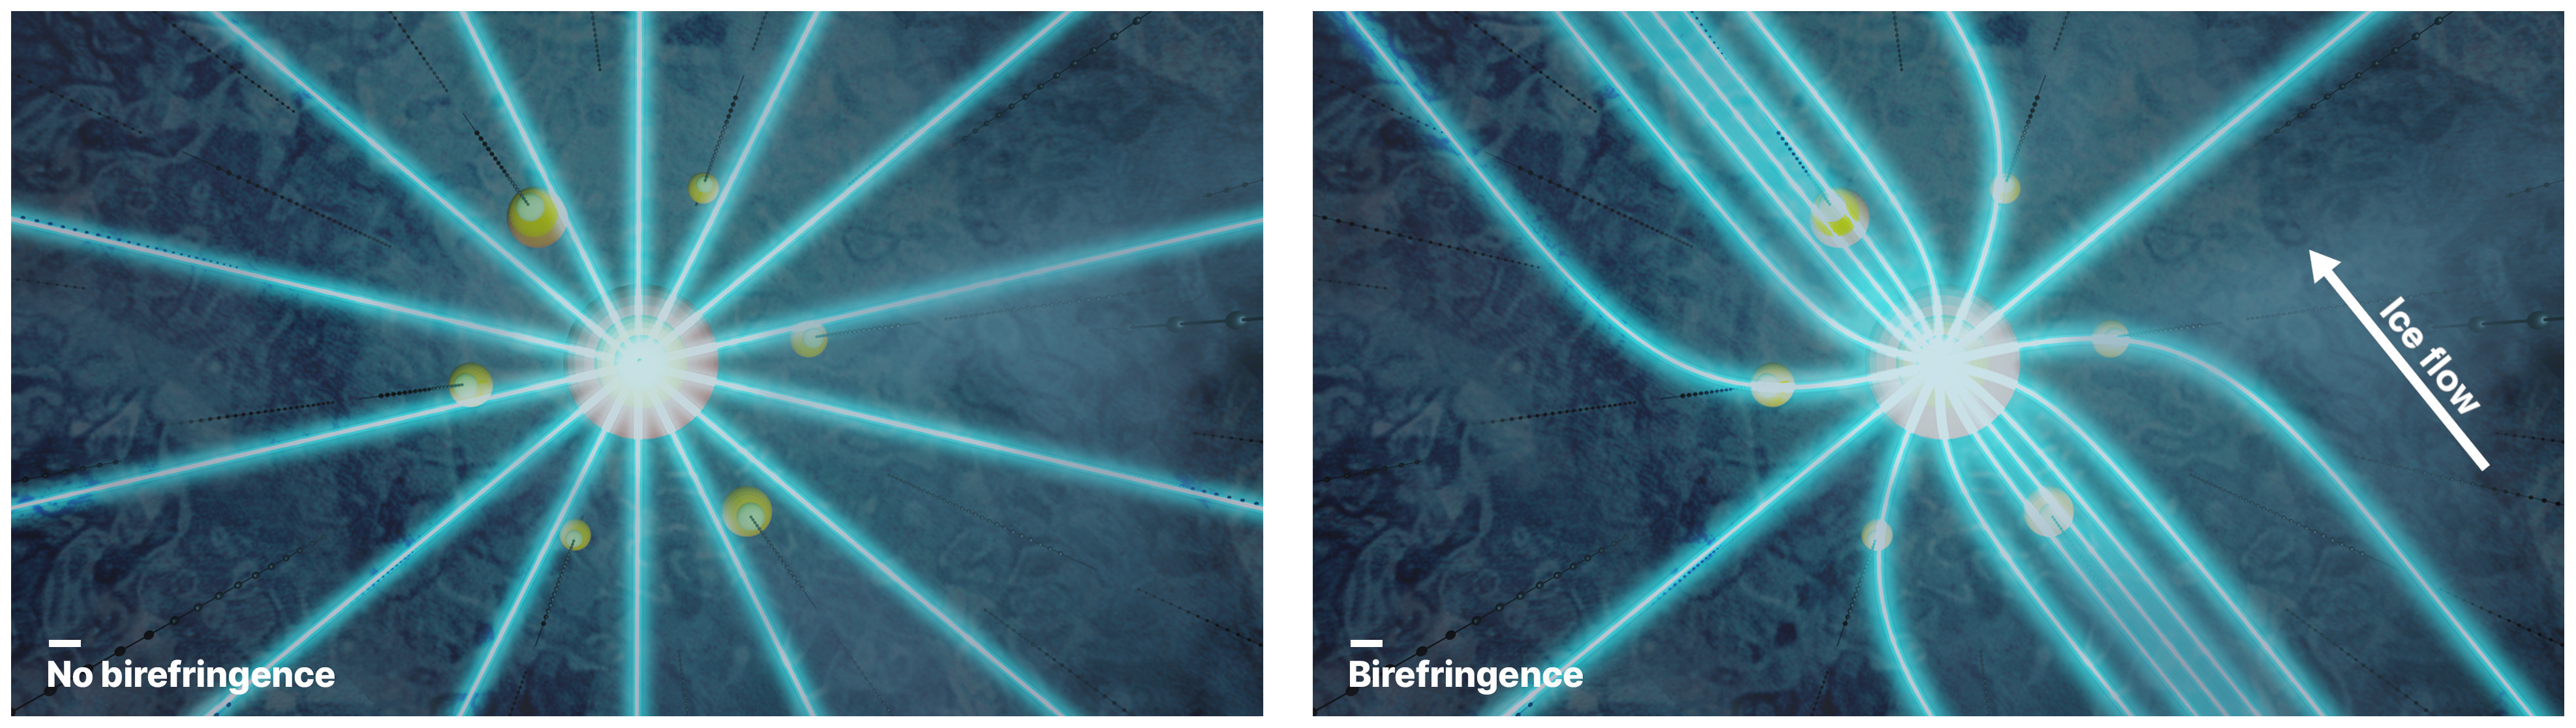
\includegraphics{./figures/nu_in_icecube/bfr_illustration.png}
	\caption{The visualisation of deflection due to birefringence. Without it (left panel), light streams out radially from an isotropic source. With this effect however (right panel), rays get deflected towards the flow axis, appearing as though photons are scattered "more" along this axis. The IceCube array around the light source can be seen as well. (Figure taken from \cite{BFR_paper})}
    \labfig{bfr_effect}
\end{figure}

The data from the dust logger also revealed that the ice layers are not perfectly horizontal; they are tilted due to the uneven surface of the bedrock \cite{dust_logger}, the so-called \textbf{ice tilt}. Initially, the effect was symmetrically parameterized along an axis (reffered to as \emph{the tilt axis}) that is approximately perpendicular to the glacial flow and also dependent on depth (same as the layers used to characterise absorption and scatetring lengths described before)\cite{spicemie}. As a result, the scattering and absorption coefficients became dependent on the full three-dimensional position in the ice rather than just the depth. A recently developed fully volumetric tilt model now includes a newly discovered tilt component along the flow \sidecite{tilt_icrc}.


Another unique property that the South Pole ice exhibits is optical \textbf{anisotropy}, a phenomenon affecting photon propagation depending on their direction relative to the "axis of anisotropy," which coincides within $\sim 1^\circ$ with the direction of the ice flow \cite{spicemie}. This effect was initially implemented as a modification to the scattering function, the only remaining Mie scattering parameter \sidecite{miescattering}, thereby changing the scattering length \sidecite{bfr_icrc2013,marcel_thesis}.  However, recent detailed studies suggest that this behavior results from diffusion within the polycrystalline ice microstructure, a previously unknown optical effect, now known as Birefringence \sidecite{bfr_icrc2019,BFR_paper}. This effect causes the ice crystals to slowly but continuously deflect towards the normal vector of the girdle plane of the crystal orientation fabric (the ice flow axis), as can be seen in \reffig{bfr_effect}.



In the context of the IceCube Detector, South Pole ice can be divided into two types: bulk ice and hole ice. Bulk ice is the undisturbed part of the ice, consisting of sheets that have formed over hundreds of thousands of years, properties of which are described above. \textbf{Hole ice}, on the other hand, is the refrozen column of ice that was melted during the deployment of the DOMs \sidecite{holeice_dima_icrc21}. This effect generally affects the forward acceptance of the IceCube DOMs. If not taken care of, it can lead to errors in directional information, therby affecting measurements involving zenith angle reconstructions of the incoming neutrino. Over the years, many efforts have been made to understand various optical properties of the South Pole ice, by fitting the LED data in terms of absorption and scattering lengths of a cherenkov photon in ice, the so-called \textbf{\emph{South Pole ICE model (SPICE model)}}. These icemodels are used in both simulation and reconstruction of the events, where particles produced in neutrino interactions are propagated (see \ref{sec:particle_propgation}) based scattering and absorption lengths described by the model. While the base model for the scattering of the photons in-ice is Mie Scattering theory \cite{miescattering} (SPICE MIE), with more dust loggers data, evolved more complex models to include, aniostropy (SPICELea), addition of tilt (SPICELea, SPICE 3.2.1), birefringence to explain anisotropy (SPICEBfr) and the latest, SPICE FTP, which includes a 2D tilt corretion in addition to birefringence. \reffig{abs_scat} shows absorption and scattering coefficients for different ice models at various depths in the detector. The corresponding scattering and absorption lengths are simply the inverse of the coefficients. It can be seen that the ice below the depth of $\sim$ 1400 m is so clear that light can travel for hundreds of meters before being absorbed. However, the light diffuses quickly, making a point-like source appear nearly isotropic at a distance of around 100 m. Effect of different icemodel corrections (specifically that of anisotropy related corrections) becomes quite relevant to reconstruct tau-neutrino events in IceCube (see Section~\ref{sec:icemodel_checks}), which is heart of the analysis presented in this thesis.


\section{Detection of Neutrinos in IceCube}
\label{sec:nu_detcetion_ic}
As described in \ref{sec:DIS}, regardless of the type of neutrino interaction (NC or CC), a variety of secondary particles are generated. In the case of a CC interaction, an accompanying charged lepton absorbs some energy, which can then undergo further decay or interact within the ice volume, leading to the production of more particles. Moreover, secondary particles, regardless of the interaction type, may also include hadrons, which are not always charged. This can, in turn, reduce the amount of \emph{visible} light in the detector. In this section, propagation of these leptons and hadrons in ice shall be explained in brief, followed by Cherenkov effect, a phenomenon by which IceCube DOMs observes these photons from the neutrino interactions. Lastly, various morphologies of these interactions will be discussed in the context of IceCube and similar detectors.

\subsection{Particle propgation in-ice}
\label{sec:particle_propgation}
When a charged particle moves through a medium like ice, it loses energy due to interactions with the medium's particles. This energy loss is characterized by the quantity $ \frac{dE}{dx} $, where $ dE $ represents the energy lost and $ dx $ the area of the medium traversed, typically measured in $\text{g/cm}^2$. Four primary processes contribute to the energy loss profile of a particle in such a medium: continuous ionization losses and radiative losses due to bremsstrahlung, pair production, and photonuclear interactions. \emph{Ionization} occurs when the particle collides with shell electrons of the atoms in the medium, causing a continuous energy loss that scales logarithmically with the particle's energy \sidecite{PDG_2024}. Additionally, if the particle is unstable, it may decay. In the context of IceCube, secondary leptons travel at nearly the speed of light, simplifying $ \beta $ to approximately 1. Thus, the decay length can be rewritten as $ \lambda_{\text{dec}} = \frac{E\tau}{mc} $, where $ E $ is the lepton's energy and $ m $ its mass. The decay length indicates the distance at which the lepton's survival probability drops to $ \frac{1}{e} \approx 36.8\% $, following the exponential decay law $ p(L) = \exp(-L/\lambda_{\text{dec}}) $.

Radiative losses, such as \emph{bremsstrahlung}, occur when the charged particle is deflected through Coulomb scattering off a target atom, while \emph{pair production} involves the creation of an electron-positron pair by an emitted photon. \emph{Photonuclear interactions} occur when a photon emitted by the particle disintegrates an atomic nucleus. These radiative losses are stochastic and scale roughly linearly with the particle's energy, with the radiation length $ X_0 $ defining the distance over which the particle’s energy decreases to $ \frac{1}{e} $ of its initial value \cite{PDG_2024}. The overall energy loss can be expressed as, 
\begin{equation}\label{eq:1}
    -\frac{dE}{dx} = a(E) + b(E)E 
\end{equation}
where $a(E)$ represents ionization losses and $b(E)$ encompasses all radiative losses.

\subsubsection{Leptons}
\label{sec:leptons_inice}
To determine a neutrino's flavor, it's important to understand the energy losses of the charged lepton created in a CC-interaction. The radiation length varies depending on the lepton's mass, influencing emitted radiation and aiding in lepton identification. For leptons with $ \beta\gamma \gg 1 $, this ionization loss can be approximated as constant, with a value of $ \langle \frac{dE}{dx} \rangle_{\text{ion}} \approx 2 \, \text{MeV/(g/cm}^2) $ \sidecite{Perkins}. In ice, this corresponds to a continuous energy loss of approximately 180 MeV per meter. However, at energies exceeding \emph{critical energy ($\mathrm{E}_\mathrm{c}$)}, radiative losses become dominant, and ionization losses become negligible, as shown in the \reffig{e_loss} \sidecite{MMC_paper}. 

For \textbf{electrons}, we mainly consider radiative losses (mainly bremsstrahlung see \reffig{e_loss}) as they are stable and do not decay. Photons from bremsstrahlung then create additional $e^+e^-$ pairs which can create more photons and so on, resulting in a cascade of particles until the energies of electrons and positrons fall below the critical level. This behavior can be described by a gamma distribution, regardless of what the initiating particle is ($e^+ \, e^- \mathrm{or} \, \gamma$) \cite{PDG_2024}. The rate of energy loss over distance can be calculated using the equation:

\begin{equation}\label{eq:2}
    \frac{dE}{dt} = E_0 b \left( \frac{(bt)^{a-1} e^{-bt}}{\Gamma(a)} \right)
\end{equation}

\begin{figure}
	\centering 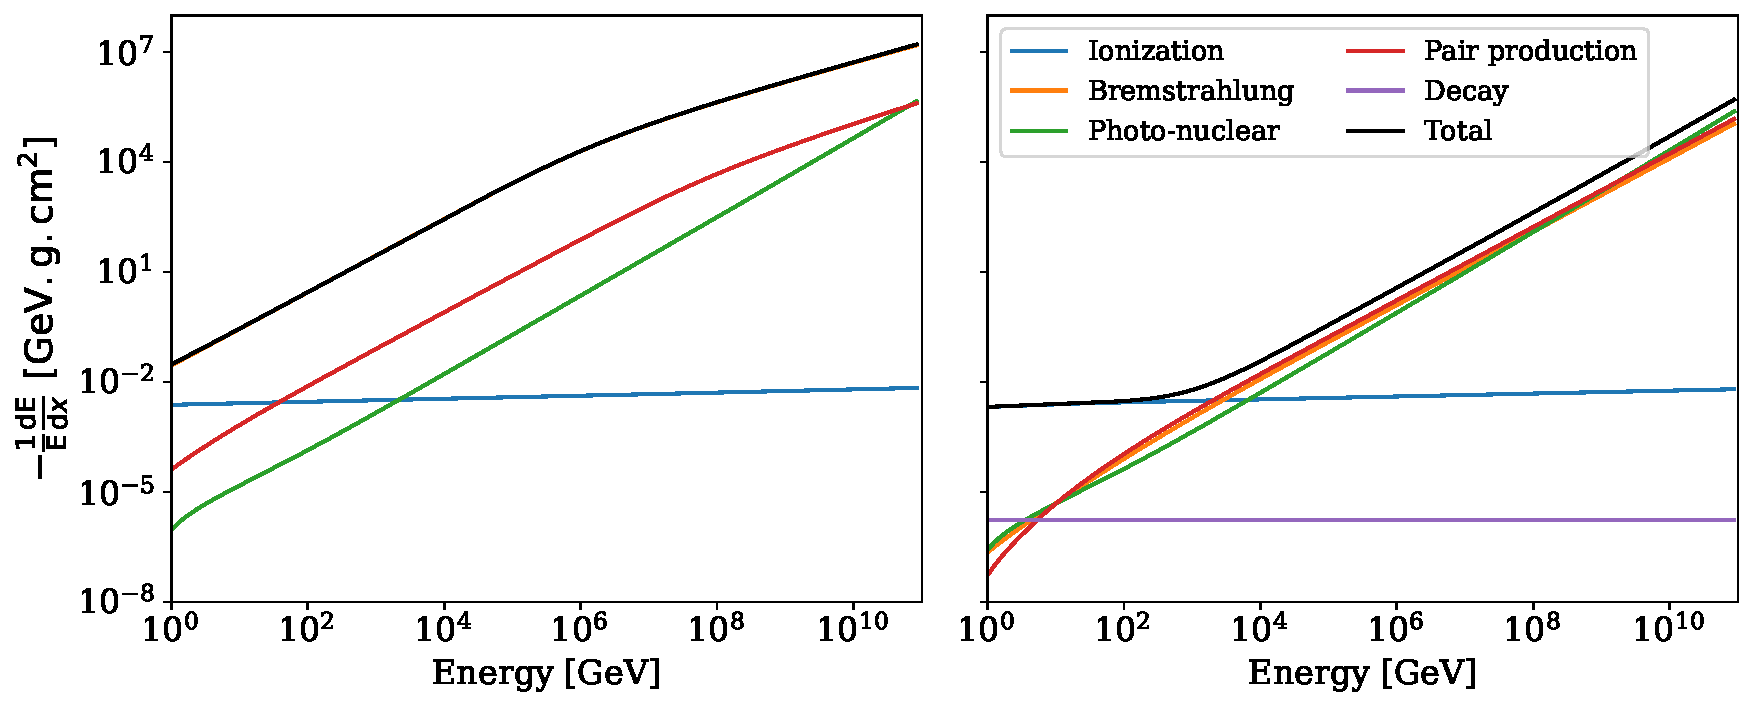
\includegraphics{./figures/nu_in_icecube/energylosses.pdf}
	\caption{The average energy loss rate per energy, for electrons (left) and muons (right) in
    ice showing the contributions from ionization, bremsstrahlung, photonuclear interactions, and pair production. Note that decay is only shown for Muons as electrons are stable particles that do not decay. Figure reproduced from \cite{MMC_paper}}
    \labfig{e_loss}
\end{figure}


Where $t$ represents the distance along the cascade in units of radiation length, and $E_0$ is the initial energy of the injected particle and $a$ and $b$ are dimensionless shower parameters. For an electromagnetic cascade induced by an electron, the parameters are $a = 2.02 + 0.63 \log(E_0/\text{GeV})$ and $b = 0.63$ (determined using \texttt{GEANT4} simulations \sidecite{shower_profile} ). The distance to the shower maximum, $t_{\text{max}}$, which is given as $t_{\text{max}}=\frac{a-1}{b}$ characterizes the size of electromagnetic cascades, indicating that they grow logarithmically in size with energy and have a characteristic size of several meters. This justifies the common approximation that light is emitted from a single point, a useful assumption for simulation and event reconstruction purposes (see Section~\ref{sec:reco} of \refch{nu_samples} for details).

At very high energies ($>10$ PeV), \emph{the Landau-Pomeranchuk-Migdal (LPM) effect} becomes significant, causing suppression of bremsstrahlung and pair production cross sections \sidecite{LPM1,LPM2,LPM3}. This suppression occurs due to destructive interference between multiple scattering centers, leading to elongated and irregular shower profiles.

\textbf{Muons} experience similar ionization and radiative losses as described in \ref{sec:particle_propagation}, but due to their larger mass, the radiation length ($\mathrm{X}_0 \sim 15 \mathrm{km}$) is much longer than that of an electron (($\mathrm{X}_0 \sim 36 \mathrm{cm}$)) of the same energy. This results in a higher critical energy ($\mathrm{E}_\mathrm{c}$) of 1 TeV in ice, allowing muons to penetrate more deeply than electrons ($\mathrm{E}_\mathrm{c}$ = 79 MeV) \cite{MMC_paper}, as can be seen in the right panel of \reffig{e_loss}. The average energy loss rate can be approximately parameterized using \ref{eq:1}, with $a = 0.00268 \mathrm{GeV}\, \mathrm{cm}^2/\mathrm{g}$ and $b = 0.47 \times 10^{-5} \, \mathrm{cm}^2/\mathrm{g}$ in ice \cite{PDG_2024}, allowing the calculation of the average range of a 1 TeV muon, which is 2 km in ice \sidenote{If one neglects these radiative losses, due to its longer lifetime ($\tau_{\mu} = 2.2\times10^{-5}$) and small mass ($m_{\mu} = 105.67$), the same energy muon will travel $\sim 6000 \mathrm{km}$ distance}.

The \textbf{tau} lepton has an even larger radiation length than a muon, $X_0 \sim 4754$ km, but its decay length is much shorter, $L_{\tau} (E_{\tau} = 1 \, \text{TeV}) = 4.9 \mathrm cm$ \cite{PDG_2024}. Thus, most taus created in IceCube will decay very promptly. $\tau^{-}$ can decay mainly via the following three modes (with the branching rations specified next to each):


\begin{equation}\label{eq:tau_decay}
    \begin{array}{rcl}
        \tau^{-} &\rightarrow& \nu_{\tau} + \text{Hadrons} \quad (64.79\%) \\
        \tau^{-} &\rightarrow& \mu^{-} + \bar{\nu}_{\mu} + \nu_{\tau} \quad (17.39\%) \\
        \tau^{-} &\rightarrow& e^{-} + \bar{\nu}_{e} + \nu_{\tau} \quad (17.82\%)
    \end{array}
\end{equation}
    
where the most commonly produced hadrons are pions and kaons \cite{PDG_2024}. Similar decay modes are observed for  $\tau^{+}$ too, by keeping in mind Lepton number conservation. Since each mode produces at least one neutrino, part of the tau lepton's energy is not "visible"\sidenote{Although these neutrinos can regenerate to interact or decay further, the probability of both neutrinos interacting within the 1 km$^3$ volume is rare}. In addition, the large radiation length will create much less light during propagation through the ice than a muon of the same energy. As will become clear in the next chapter, a 1 TeV tau cannot be distinguished from an electron due to its short decay length and the large sensor spacing of IceCube. Taus from $\nu_{\tau}$ charged-current interactions are polarized \sidecite{Carlos_Taupolarisation}, and due to the small decay length and large radiation length, the decay products' energy spectrum gets affected. This becomes important in the analysis presented in this thesis, where one of the observables is an estimate of deposited energy in the detector, see Section~\ref{sec:tau_polarisation} for details.


\subsubsection{Hadrons}
\label{sec:hadrons_inice}
\textbf{Hadrons} are produced in all flavour NC interactions, or when a tau lepton decays (see \ref{eq:tau_decay}). Hadronic cascades are more complex than electromagnetic cascades because they involve a wider variety of secondary particles and have larger uncertainties in the relevant cross-sections. Unlike electromagnetic cascades that consist solely of electrons, positrons, and photons, hadronic cascades involve numerous neutral particles that do not emit "\emph{visible}" light in the detector, resulting in a lower light yield (see \ref{sec:cherenkov}). Additionally, the production threshold for hadrons is higher compared to that for electrons, positrons, and photons \sidecite{MMC_paper}. Despite these differences, a significant portion of the cascade’s total energy can still be carried by electrons, positrons, and photons, which are produced by electromagnetic sub-cascades initiated by the decay of neutral pions ($\pi^0 \rightarrow \gamma\gamma$). 

The longitudinal profile of hadronic showers can be parameterized using \ref{eq:2}, although the specific values for the shower parameters are $a = 1.81 + 0.39 \log(E_0/\text{GeV})$ and $b = 0.34$ (assuming cascade is induced by a charged pion). It is important to note that the electromagnetic radiation length used in these equations applies to both types of cascades; however, it does not account for the generally larger nuclear interaction length characteristic of hadronic showers, adding another layer of complexity and resulting in greater fluctuations in the overall development of the particle cascade. This makes modeling hadronic cascades more challenging compared to their electromagnetic counterparts.

\subsection{Cherenkov effect}
\label{sec:cherenkov}

\begin{marginfigure}
    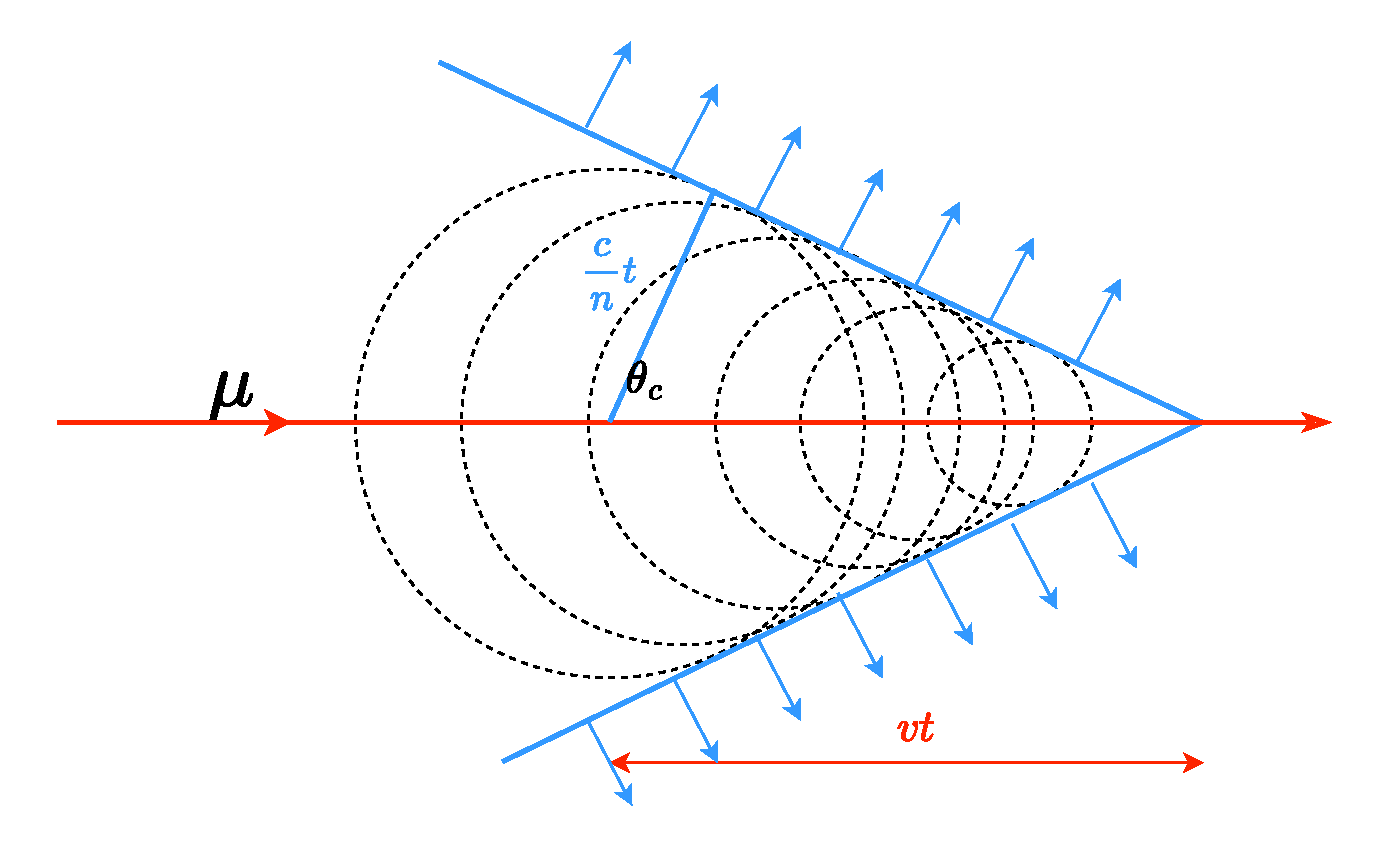
\includegraphics{./figures/nu_in_icecube/Cherenkov.pdf}
    \caption{The sketch shows the Cherenkov effect for a muon traveling through a dielectric medium with a velocity $v = \beta c$ (in red). The medium has a refractive index $n$, and the phase velocity of light $v_\mathrm{phase} = \frac{c}{n} $(in blue). The circles in the sketch represent wavefronts with equal phase shifts and illustrate isotropic and coherent emission (blue arrows) at an angle $\theta_c$ , for $v>v_\mathrm{phase}$.}
    \labfig{cherenkov}
\end{marginfigure}

When a charged particle moves through a medium at speed exceeding the phase velocity of light in that medium, it emits \emph{Cherenkov radiation} \sidecite{Cherenkov}, much like the shock wave generated by a supersonic jet. This radiation is emitted in a cone at an angle $\theta_C = \cos^{-1}\left(\frac{1}{\beta n}\right)$ relative to the particle's direction of travel, where $n$ is the refractive index of the medium and $\beta = \frac{v}{c}$ represents the ratio of the particle's velocity to the speed of light in a vacuum (see \reffig{cherenkov}). In ice, with a refractive index of $n = 1.31$ at a wavelength of 400 nm, which corresponds to the peak sensitivity of IceCube's optical modules (see, \ref{sec:dom}), the emission threshold for Cherenkov radiation is $\beta_\text{Ch} \gtrsim 0.76$. This corresponds to a minimum energy of 0.28 MeV for electrons and 58.09 MeV for muons, both of which are below IceCube's detection threshold of around 200 GeV. For high-energy particles in IceCube, where $\beta \simeq 1$, the Cherenkov cone's opening angle is $\theta_\text{Ch} \simeq 40.2^\circ$ at the peak sensitivity wavelength. The number of Cherenkov photons emitted within a waveband $d\lambda$ by a particle with charge $ze$ within the propagation length $dx$ is given by the Frank-Tamm formula \sidecite{Frank_Tamm}:

\begin{equation}\label{eq:cherenkov_ph}
    \frac{d^2N}{dxd\lambda} = \frac{2\pi \alpha z^2}{\lambda^2} \left( 1 - \frac{1}{\beta^2 n(\lambda)^2} \right)
\end{equation}
where, $\alpha$ is fine structure constant \sidecite{PDG_2024}. Using this formula, one can calculate that for a high-energy particle with $\beta \simeq 1$ passing through ice, approximately 250 photons/cm are emitted in the wavelength range of 300 nm to 500 nm, which is within IceCube's optimal detection range \sidecite{shower_profile}. 

Neutrino interactions in IceCube are detected indirectly through Cherenkov radiation from secondary charged particles (leptons, hadrons and electromagnetic showers, see \ref{sec:particle_propgation}) , reffered to as \emph{visible light} in IceCube. At energies above 1 TeV, the Cherenkov light from a muon itself becomes negligible, and detection primarily depends on light emitted by secondary particle showers along the muon's path. 

\subsection{Event Signatures}
\label{sec:morphologies}
The previous sections described the detector and its various components, along with the interactions and passage of neutrinos and the secondary particles they produce. In IceCube, events are visualized with the detector shown as an array of strings, with each colored sphere representing a triggered DOM. The sphere's size scales with the detected cherenkov light amount (charge accumulated), and its color indicates the arrival time. Section \ref{sec:DIS}, discussed how all-flavor neutral current (NC) interactions result in the transfer of a fraction of the neutrino's energy to the nucleus, initiating a hadronic shower. On the other hand, charged current (CC) interactions are accompanied by a charged lepton, whose propagation patterns were detailed in \ref{sec:leptons_inice}. The involvement of specific neutrino flavors in CC events leads to a distinct energy deposition patterns (\emph{morphology}), which can be used to identify the neutrino flavor. Additionally, when a neutrino interaction occurs within the volume of the detector, it is classified as a \emph{starting} event, and if the energy deposition is entirely within the detector volume, it is termed a \emph{contained} event.
Hadrons and electrons produce showers, which are known in IceCube as \textbf{cascades}. Due to the low radiation lengths of electrons and the short shower maximum caused by various secondary particles, cascades are contained within a few meters. This causes Cherenkov light emission to appear as a point-like source relative to the kilometer-scale detector. However, due to a higher scattering coefficient \ref{sec:icemodel} the light pattern appears almost spherical for cascades see \reffig{topologies}, due to which, the angular information is lost (or becomes less reliable) upon reaching the DOMs, leading to a poor angular resolution. In electromagnetic cascades, most of the interaction energy is contained within the cascade, making $\nu_{e}$ - CC events excellent candidates for energy estimation \sidecite{energy_reco}.
\begin{figure}
	\centering 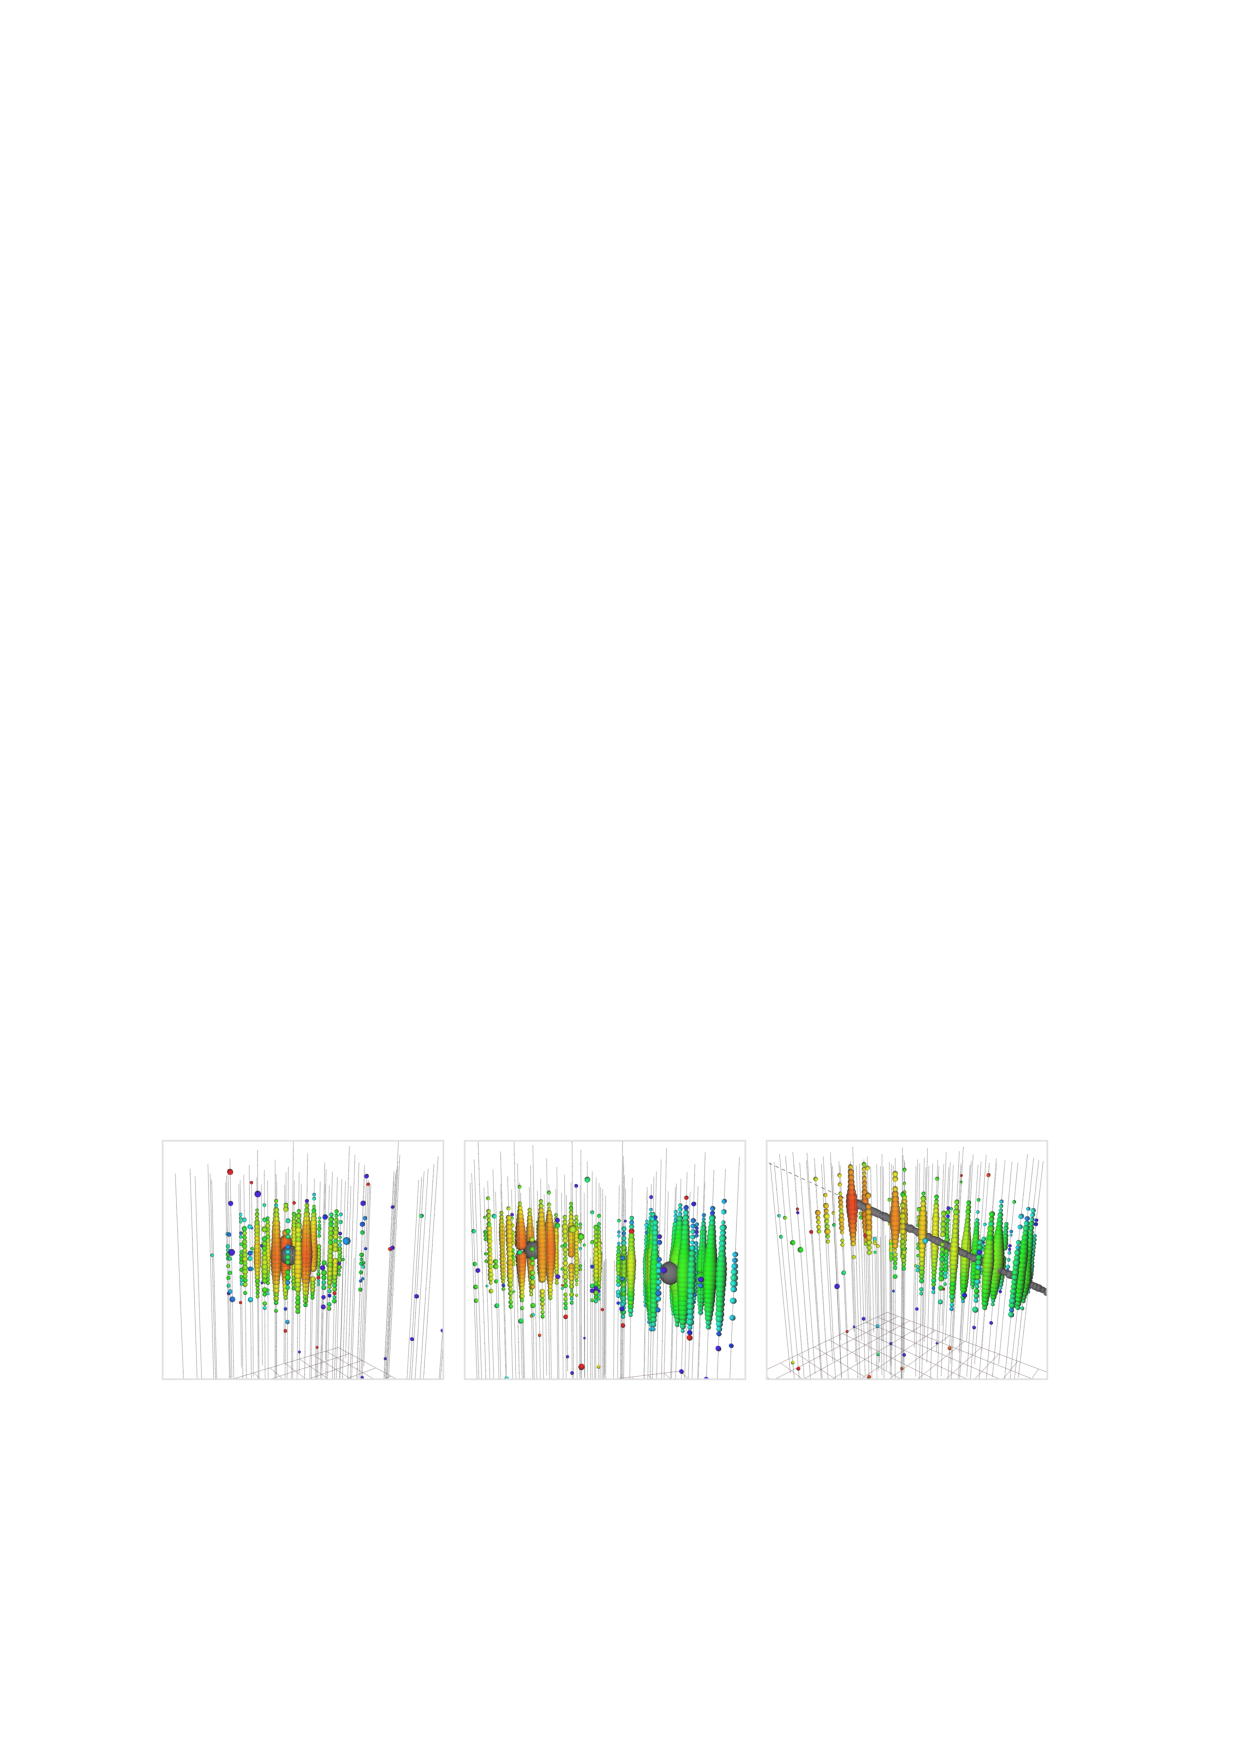
\includegraphics{./figures/nu_in_icecube/topologies.pdf}
	\caption{Simulated event signatures of single cascade (left), double cascade (middle), and track (right). Sizes of the spheres represent the amount of detected light, and colors show the photon arrival times. Single cascades are caused by electromagnetic and hadronic showers, double cascades by the production and decay of a tau lepton, and tracks by muons traversing the detector.}
    \labfig{topologies}
\end{figure}

\textbf{Tracks} are observed when highly energetic muons traverse the detector, most commonly from atmospheric muons produced by cosmic-ray-induced air showers. Tracks are also caused by CC interactions of $\nu_{\mu}$($\bar{\nu}_\mu$), which produce a hadronic cascade and a $\mu^-$ ($\mu^+$). When the neutrino interaction vertex is outside the detector volume, atmospheric muons and neutrino-induced muons are indistinguishable unless their energy and direction are considered\todo{is there any nu sources paper that can be cited for this claim?}, leading to \emph{a through-going track}. When the vertex is inside the detector volume, both the hadronic cascade and the emerging muon track are visible, resulting in \emph{a starting track}, which can only be caused by neutrino interactions. Although muons exhibit stochastic energy loss and are likely to exit the detector, resulting in poor energy resolution, the light deposition along an extended path (see \reffig{topologies}) provides good angular resolution (less than 1 degree), making tracks ideal for identifying high-energy astrophysical sources \cite{energy_reco}.

Tau neutrinos in IceCube exhibits variety of signatures, thanks to different tau decay modes (\ref{eq:tau_decay}). This leads to various event morphologies \sidecite{Tau_int_inice} based on factors like position of both, the neutrino interaction and tau decay verteces, decay channel and the decay length, as shown in \reffig{tau_morphologies}. The tau decay length ($\mathrm{L}_\tau$) is connected to Energy of tau lepton ($E_{\tau}$) via $\mathrm{L}_{\tau}\simeq\frac{50\mathrm{m}}{1\mathrm{PeV}}E_{\tau}$. $\nu_{\tau}$ CC events typically produce two energy depositions: an initial interaction cascade followed by a tau decay product, which can be a track or cascade, depending on the decay channel. The muonic decay channel results in a dim tau track followed by a brighter muon track.\footnote{The stochasticity of muon energy losses and the low branching ratio of the muonic decay channel (17.4\%) make it challenging to search for this signature. Therefore, this decay channel is excluded from the analysis presented in this thesis.} The other decay channels, involving hadrons or electrons, produce a cascade, leading to the so-called \textbf{double bang} events \sidecite{double_bang}. Around 59\% of tau-neutrino interactions are double bang events.\footnote{The muonic decay of the tau has a branching ratio of around 17\%, while all other decay channels of the tau produce another cascade with an inclusive branching ratio of approximately 83\%. When multiplied by the fraction of the charged-current cross-section over the total cross-section \cite{PDG_2024}, about 59\% of all tau-neutrino interactions are double bang events.}

\begin{figure}
	\centering 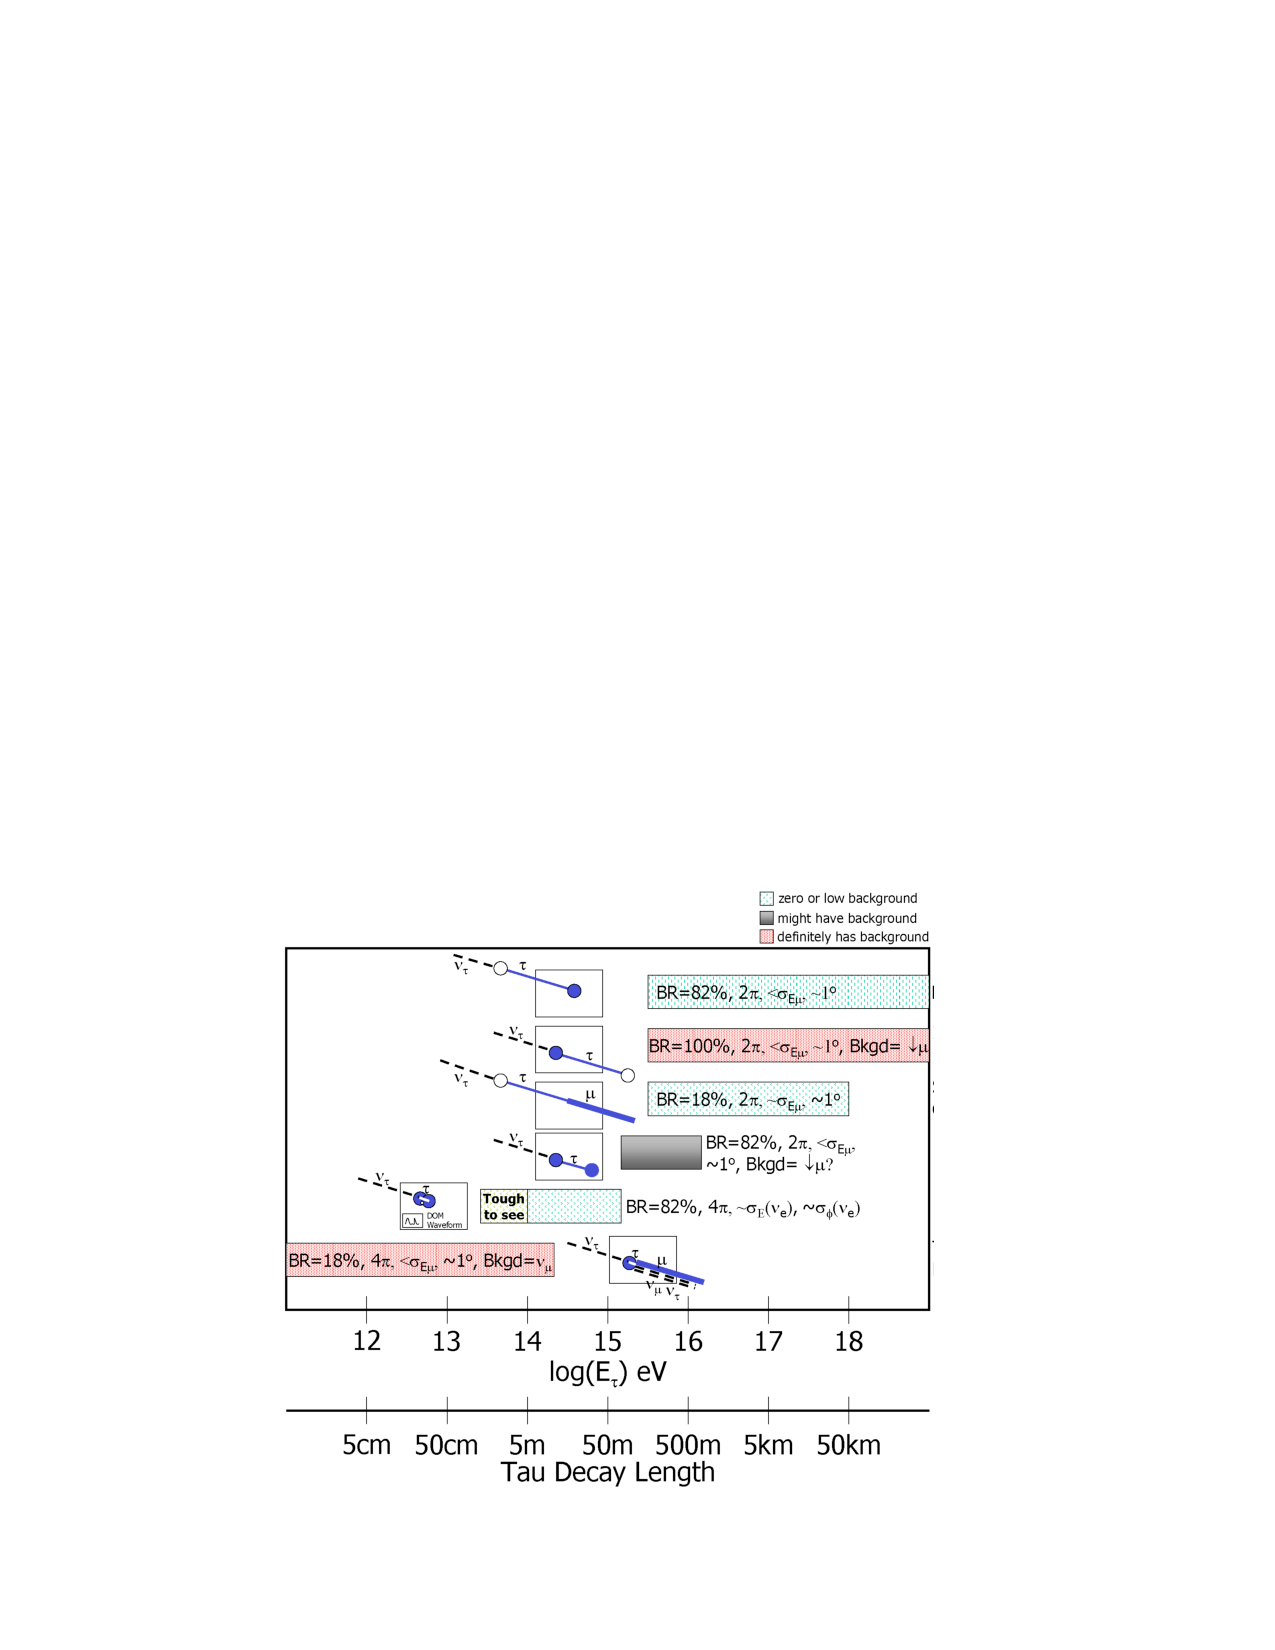
\includegraphics{./figures/nu_in_icecube/tau_interactions.pdf}
	\caption{Various morphologis of $\nu_{\tau}$ cc events in IceCube, as a function of $E_{\tau}$ and $\mathrm{L}_\tau$. Circle represent a cascade, dotted line represents primary $\nu_{\tau}$, thin line, Tau lepton track and thick line represent muon track.(Figure taken from \cite{Tau_int_inice})}
    \labfig{tau_morphologies}
\end{figure}

These double bang events are further classified based on whether both the interaction vertex and tau decay vertex are within the detector volume (see \reffig{tau_morphologies}). At lower energies (below $(\sim 100$) TeV), the separation between the two cascades is small, making them difficult to resolve. In some cases, if the event occurs close to a string or Digital Optical Module (DOM), two distinct time-connected pulses can be observed, known as the \textbf{double pulse} technique. However, identifying tau neutrino events in IceCube is challenging due to background muons and the difficulty in reconstructing such events. Recent developments using CNN classifiers have identified seven astrophysical tau neutrino candidates \sidecite{CNN_tau}. Lastly, if both of these caascades are contained in the active volume, and they are far enough to be reconstructed reliably, the morphology is called \textbf{double cascade}. This method has low and high tau energy threshold, since below certain energy ($\sim100$ TeV) the decay length is quite short, making them indistinugishable from a usual cascade event, and energies above 10 PeV, (where theoretically  the length should be  large enough to separate the two cascades) one of the cascades will always be outside the detector volume. In such case, a larger detector volume, such as in IceCube Gen2, could extend the energy range for identifiable double cascade events (see \refch{gen2}). 

The analysis performed in this thesis aims to measure neutrino flavour composiition where three of the morphologies explained above, starting tracks, double cascades and cascades (from hereon reffered to as single cascades, to differentiate from double) are used to identify flavour of the neutrino. Double cascades are not only challanging due to their tricky geometry but also because of involvement of both electromagnetic and hadronic particle showers involved. Lastly, as was discussed in \ref{sec:icemodel }the medium (ice) itself has many characteristic properties that affects the reconstruction of these events drastically. Details of sampling these high energy starting events and reconstructing them in to these three morphologies will be explained in the next chapter. 






% \begin{table*}[h!]
%     % \centering
%     \caption{Table showing the interaction types, flavors, morphologies, and containment types.}
%     \begin{tabular}
%     \hline
%     \textbf{Interaction Type} & \textbf{Flavor} & \textbf{Morphology} & \textbf{Containment Type} \\ \hline
%     \multirow{2}{*}{Neutral Current (NC)} & All & Hadronic Cascade & Starting, Contained \\  
%      &  &  &  \\ \hline
%     \multirow{10}{*}{Charged Current (CC)} & $\nu_e$ & Electromagnetic Cascade & Starting, Contained \\ \cline{2-4} 
     
%      & $\nu_\mu$ &  Track &  Starting\\ 
%      &  &  & Through-going \\ \cline{2-4} 
%      & $\nu_\tau$ & Tau Track & Starting, Contained \\ \cline{2-4} 
%      &  & Double Bang & Starting, Contained \\ \cline{2-4} 
%      &  & Dim Tau Track, Bright Muon Track & Starting, Contained \\ \cline{2-4} 
%      &  & Double Cascade & Starting, Contained \\ \cline{2-4} 
%      &  &  &  \\ \hline
%     \end{tabular}
    
% \end{table*}
    